%%==================================================
%% chapter02.tex for SJTU Master Thesis
%% based on CASthesis
%% modified by wei.jianwen@gmail.com
%% Encoding: UTF-8
%%==================================================


%%%%%%%%%%%%%%%%%%%%%%%%%%%%%%%%%%%%%%%%%%%%%%%%%%%%%
%%
%%      可搜索加密技术
%%
%%%%%%%%%%%%%%%%%%%%%%%%%%%%%%%%%%%%%%%%%%%%%%%%%%%%%
\chapter{对称可搜索加密技术} %%预备知识
\label{chap:search}


%%%%%%%%%%%%%%%%%%%%%%%%%%%%%%%%%%%%%%%%%%%%%%%%%%%%%
%%
%%      基本知识介绍
%%
%%%%%%%%%%%%%%%%%%%%%%%%%%%%%%%%%%%%%%%%%%%%%%%%%%%%%
\section{预备知识}
\label{sec:search_symm_basic}

\subsection{\textbf{数学基础知识}}
\label{sec:search_symm_math_knowledge}


%%%%%%%%%%%%%%%%%%%%%%%%%%%%%%%%%%%%%%%%%%%%%%%%%%%%%%%%%%%%%%%%%%%%%%
\begin{defn}[可忽略函数(Negligible Function)]
\label{defn:ignore_function}

对于一个函数$f$ : $N^* \rightarrow N^*$,如果对任意给定的正多项式$p(.)$,总存在一个足够大的数$k$,
使$f(k) < \frac{1}{p(k)}$,则称函数$f$在$k$上是可忽略的。

\end{defn}
%%%%%%%%%%%%%%%%%%%%%%%%%%%%%%%%%%%%%%%%%%%%%%%%%%%%%%%%%%%%%%%%%%%%%%


%%%%%%%%%%%%%%%%%%%%%%%%%%%%%%%%%%%%%%%%%%%%%%%%%%%%%%%%%%%%%%%%%%%%%%
\begin{defn}[伪随机函数(Pseudo-random Function)\cite{bellare1996pseudorandom}]
\label{defn:psedu_random_function}

对任意的函数$\mathcal{F} : \{0,1\}^n * \{0,1\}^k \rightarrow \{0,1\}^m$,如果满足:
\begin{enumerate}
  \item
  对于任意给定的输入$K \in \{0,1\}^k$和$x \in \{0,1\}^n$,$\mathcal{F}(x,K)$总能在多项式时间内被计算;

  \item
  对所有多项式大小的敌手$\mathcal{A}$,有:
  \begin{center}
  $|Pr[\mathcal{A}^{\mathcal{F}_K(.)} = 1 : K \overset{\$}{\leftarrow} \{0,1\}^k] - Pr[\mathcal{A}^{\mathcal{G}(.)} = 1 : \mathcal{G} \overset{\$}{\leftarrow} Func[n,m]]| \leq negl(k) $
  \end{center}
($Func[n,m]$表示所有$\{0,1\}^n \rightarrow \{0,1\}^m$的函数集合,$negl$是在$k$上的可忽略函数)。

\end{enumerate}
则称函数$\mathcal{F}$是伪随机函数。如果函数$\mathcal{F}$是双射,则称为伪随机置换函数。

\end{defn}
%%%%%%%%%%%%%%%%%%%%%%%%%%%%%%%%%%%%%%%%%%%%%%%%%%%%%%%%%%%%%%%%%%%%%%



%%%%%%%%%%%%%%%%%%%%%%%%%%%%%%%%%%%%%%%%%%%%%%%%%%%%%%%%%%%%%%%%%%%%%%
\begin{defn}[伪随机生成器(Pseudo-random Generator)\cite{haastad1999pseudorandom}]
\label{defn:pseudo_random_generator}
对任意函数$\mathcal{G}: \{0,1\}^n \rightarrow \{0,1\}^m$,在$m > n$的条件下,如果满足:
\begin{enumerate}
    \item
    函数$\mathcal{G}$可以使用确定性的算法在多项式时间内被计算;

    \item
    对所有$t$多项式时间的算法$\mathcal{A}$,有:
    \begin{center}
    $|Pr[\mathcal{A}(\mathcal{G}(s)) = 0 | s \overset{\$}\leftarrow \{0,1\}^n] - Pr[\mathcal{A}(r) = 0 | r \overset{\$} \leftarrow \{0,1\}^m]| < negl(k)$。
    \end{center}

\end{enumerate}
则称函数$\mathcal{G}$是在条件$(t,negl(k))$下的伪随机生成器($negl$是在$k$上的可忽略函数)。
在多项式时间内,伪随机生成器$\mathcal{G}$输出的字符串与随机字符串不可区分。
\end{defn}
%%%%%%%%%%%%%%%%%%%%%%%%%%%%%%%%%%%%%%%%%%%%%%%%%%%%%%%%%%%%%%%%%%%%%%


%%%%%%%%%%%%%%%%%%%%%%%%%%%%%%%%%%%%%%%%%%%%%%%%%%%%%%%%%%%%%%%%%%%%%%%%
%%\begin{defn}[多项式时间算法]
%%\label{defn:multi_time_function}
%%%\textbf{定义 2.4(多项式时间算法):}
%%
%%对于输入规模为n的算法,如果在最差情况下的运行时间为$O(n^{l})$ ($l$为常数),则称其为多项式时间算法。
%%\end{defn}
%%%%%%%%%%%%%%%%%%%%%%%%%%%%%%%%%%%%%%%%%%%%%%%%%%%%%%%%%%%%%%%%%%%%%%%%



%%%%%%%%%%%%%%%%%%%%%%%%%%%%%%%%%%%%%%%%%%%%%%%%%%%%%%%%%%%%%%%%%%%%%%
%%\begin{defn}[向量空间]
%%\label{defn:schmidt_normalize}
%%给定域$F$, $F$上的集合$V$,如果满足以下两种运算: \\
%%\ \ \textbf{. 向量加法:} $V + V  \rightarrow V$,将$V$中两元素映射到$V$集合中;  \\
%%\ \ \textbf{. 标量乘法:} $F * V  \rightarrow V$,分别将$F$和$V$中元素映射到$V$中一元素。 \\
%%则集合$V$称作域$F$上的向量空间。
%%数域$F$上一个有序的n元数组称为其上的一个n维向量,该向量表示为:$(a_1, a_2, ..., a_n)$,
%%$a_i$表示向量的第i个元素。
%%\end{defn}
%%%%%%%%%%%%%%%%%%%%%%%%%%%%%%%%%%%%%%%%%%%%%%%%%%%%%%%%%%%%%%%%%%%%%%




%%%%%%%%%%%%%%%%%%%%%%%%%%%%%%%%%%%%%%%%%%%%%%%%%%%%%%%%%%%%%%%%%%%%%%%
%\begin{defn}[施密特正交化]
%\label{defn:schmidt_normalize}
%%\textbf{定义 2.5(施密特正交化):}
%
%设 $\boldsymbol{v} \in \boldsymbol{V^n}$,$\boldsymbol{V}^k$是$\boldsymbol{V}^n$上的$k$ 维子空间,$\boldsymbol{v}$上标准正交基为$\{ \boldsymbol{\eta}_1,\ldots, \boldsymbol{\eta}_k \}$,且$\boldsymbol{v}$不在$\boldsymbol{V}^k $ 上。由投影原理知,$\boldsymbol{v}$与其在$\boldsymbol{V}^k$上的投影$\mathrm{proj}_{\boldsymbol{V^k}} \boldsymbol{v}$ 之差 $\boldsymbol{\beta} = \boldsymbol{v} -  \sum_{i=1}^{k}\mathrm{proj}_{\boldsymbol{\eta}_i}\,\boldsymbol{v}$ = $\boldsymbol{v} - \sum_{i=1}^{k}\langle \boldsymbol{v}, \boldsymbol{\eta}_i \rangle \boldsymbol{\eta}_i$正交于子空间$\boldsymbol{V}^k$,即$\boldsymbol{\beta}$正交于$\boldsymbol{V}^k$的正交基$\boldsymbol{\eta}_i$。将$\boldsymbol{\beta}$单位化:$\boldsymbol{\eta}_{k+1} = \frac{\boldsymbol{\beta}}{\|\boldsymbol{\beta}\|} = \frac{\boldsymbol{\beta}}{\sqrt{\langle \boldsymbol{\beta},\boldsymbol{\beta} \rangle }}$,那么$\{ \boldsymbol{\eta}_1,\ldots, \boldsymbol{\eta}_{k}, \boldsymbol{\eta}_{k+1}\}$就是$\boldsymbol{V}^k$在$\boldsymbol{v}$上扩展的子空间$\mathrm{span}\{\boldsymbol{v},\boldsymbol{\eta}_1,...,\boldsymbol{\eta}_k\}$的标准正交基。
%
%对于向量组$\{ \boldsymbol{v}_1,\ldots, \boldsymbol{v}_{m} \}$张成的空间$\boldsymbol{V}^m (m<n)$,只要从其中一个向量 $\boldsymbol{v}_1$ 所张成的一维子空间 $\mathrm{span}\{\boldsymbol{v}_1\}$ 开始,重复上述扩展构造正交基的过程,就能够得到在$\boldsymbol{V}^n$ 的一组正交基,则称该向量正交化的过程为Gram-Schmidt正交化。
%\end{defn}
%%%%%%%%%%%%%%%%%%%%%%%%%%%%%%%%%%%%%%%%%%%%%%%%%%%%%%%%%%%%%%%%%%%%%%%


%\subsection{\textbf{密码学基础知识}}
%\label{sec:search_symm_cryptology_knowledge}


%%%%%%%%%%%%%%%%%%%%%%%%%%%%%%%%%%%%%%%%%%%%%%%%%%%%%%%%%%%%%%%%%%%%%%%%
%%\begin{defn}[随机预言机]
%%\label{defn:random_oracle}
%%
%%预言机\cite{bellare1993random}是一个具有预言的图灵机,由四元组$M$ = $\langle Q, \delta, q_0, F \rangle$ 构成:
%%\begin{itemize}
%%  \item
%%  $Q$ 是有限多个状态的集合;
%%
%%  \item
%%  $Q \times \{B,1\}^2 \rightarrow Q \times \{B,1\} \times \{L,R\}^2$是转移函数,$L$和$R$分别代表左移和右移;
%%
%%  \item
%%  $q_0 \in Q$ 代表起始状态;
%%
%%  \item
%%  $F \subseteq Q$ 是终止状态的集合。
%%\end{itemize}
%%如果预言机满足以下性质:
%%\begin{itemize}
%%  \item
%%  确定性:对于相同的输入,预言机产生相同的输出;
%%
%%  \item
%%  均匀性:预言机的取值在输出空间中均匀分布;
%%
%%  \item
%%  有效性:对于任意给定的输入,预言机都能在低阶多项式内完成。
%%\end{itemize}
%%则称预言机为随机预言机。
%%
%%\end{defn}
%%%%%%%%%%%%%%%%%%%%%%%%%%%%%%%%%%%%%%%%%%%%%%%%%%%%%%%%%%%%%%%%%%%%%%%%


%%%%%%%%%%%%%%%%%%%%%%%%%%%%%%%%%%%%%%%%%%%%%%%%%%%%%%%%%%%%%%%%%%%%%%
\begin{defn}[对称加密方案]
\label{defn:random_oracle}
对称加密方案$SKE$是由三个多项式时间算法组成的集合,定义:$SKE$ =($Gen$, $Enc$, $Dec$)。
\begin{itemize}
  \item
  \textbf{$Gen$:}输入安全参数$k$,返回私钥$K$;

  \item
  \textbf{$Enc$:}输入密钥$K$和明文消息$m$,并返回密文$c$;

  \item
  \textbf{$Dec$:}输入密钥$K$和密文$c$(密钥$K$与密文$c$生成时的密钥相同),解密得到消息$m$。

\end{itemize}
\end{defn}
%%%%%%%%%%%%%%%%%%%%%%%%%%%%%%%%%%%%%%%%%%%%%%%%%%%%%%%%%%%%%%%%%%%%%%

\begin{defn}[$PCPA$-安全]
\label{defn:pcpa_security}
如果$SKE$ =($Gen$, $Enc$, $Dec$)是一个对称加密方案,$\mathcal{A}$是一个敌手,
在下面的概率实验$PCPA_{SKE,\mathcal{A}}(k)$过程中:
\begin{enumerate}
  \item $Gen(1^k )$生成一个密钥$K$,
	
  \item $\mathcal{A}$被赋予oracle访问$Enc_K($.$)$的能力,
	
  \item $\mathcal{A}$输出一条信息$m$,
	
  \item 首先$c_0 \leftarrow Enc_K(m)$和$c_1 \overset{\$} \leftarrow \mathcal{C}$分别产生两个密文$c_0$和$c_1$,
  这里$\mathcal{C}$表示$SKE$方案的整个密文空间。然后随机的选择$b \overset{\$}\leftarrow \{0,1\}$,并发送$c_b$给敌手$\mathcal{A}$,
	
  \item $\mathcal{A}$被再次给予访问加密oracle的能力,经过多项式次数的查询后输出一个$b'$,
	
  \item 如果$b'=b$,该实验返回1,否则返回0。

  \end{enumerate}

  如果对于所有的多项式敌手$\mathcal{A}$,有:
  \begin{center}
  $Pr[PCPA_{SKE,A}(k)=1] \leq 1/2 + negl(k)$
  \end{center}
  这里的概率仅与$b$的选择和算法$Gen$与$Enc$引入的随机量有关,
  则我们认为$SKE$方案是$CPA$-安全的。
\end{defn}


%%
%%%%%%%%%%%%%%%%%%%%%%%%%%%%%%%%%%%%%%%%%%%%%%%%%%%%%%%%%%%%%%%%%%%%%%%%
%%\begin{defn}[自信息I]
%%\label{defn:information}
%%%\textbf{定义 2.6(消息):}
%%
%%对于一离散性随机实验,其各实验结果为独立的随机分布: $ S \in {s_1,s_2,s_3...} 且 p(S=s)= p_k$,$ \sum_{k}p_k = 1 $,故事件 $S = s_k$, 出现概率为 $p_k$ 的消息量为:
%%\begin{equation*}
%%  I(S_k) = log_2(\frac{1}{p_k}) = -log_2(p_k)
%%\end{equation*}
%%
%%\end{defn}
%%%%%%%%%%%%%%%%%%%%%%%%%%%%%%%%%%%%%%%%%%%%%%%%%%%%%%%%%%%%%%%%%%%%%%%%
%%
%%%%%%%%%%%%%%%%%%%%%%%%%%%%%%%%%%%%%%%%%%%%%%%%%%%
%%\begin{defn}[信息熵]
%%\label{defn:information_entropy}
%%%\textbf{定义 2.7(信息熵):}
%%
%%对一个值域为 $\{x_1, x_2, ..., x_n \}$ 的随机变量 $X$ 的熵值 H 定义为:
%%\begin{equation*}
%%H(X)  =  E(I(X))
%%\end{equation*}
%%
%%其中,E 代表了期望函数,而 $I(X)$ 是 $X$ 的信息量(又称为信息本)。$I(X)$ 本身是个随机变量。如果 p 代表了 X 的随机概率分布函数(probability function),则熵的公式可以表示为:
%%\begin{equation*}
%%  H(X) = \sum_{i=1}^n {p(x_i)\,I(x_i)} = -\sum_{i=1}^n {p(x_i) \log_b p(x_i)}
%%\end{equation*}
%%
%%\end{defn}
%%%%%%%%%%%%%%%%%%%%%%%%%%%%%%%%%%%%%%%%%%%%%%%%%%%%%%%%%%%%%%%%%%%%%%%%





\subsection{\textbf{安全索引}}
\label{sec:search_symm_secure_index}
\begin{enumerate}
  \item \textbf{正向安全索引(Forward-Index)}\\
  Goh.等在\cite{goh2003secure}中给出了一种可搜索加密方案,是第一篇使用索引结构的方案。
  该方案使用Bloom Filter\cite{gremillion1982designing}建立正向的索引结构,从而加快单词在文章中的查找。
  正向索引是一种使用文档映射到对应单词集的二元组结构,即针对每个文档保存一份包含所有单词的集合,
  例如表\ref{tab2-1}所示:

  \begin{table}[!hbt]
  \centering
  \begin{tabular}[t]{|c|c|}
  \hline
    文档 &       单词 \\
    \hline
    $D1$ & hello, word, welcome, document \\
    \hline
    $D2$ & hello, paper, good, well \\
    \hline
    $D3$ & world, paper, welcome, good \\
    \hline
    $D4$ & document, welcome, well  \\
    \hline
  \end{tabular}
  \bicaption[tab2-1]{正向索引示例}{正向索引示例} {Table}{An Example Of Forward-Index}
  \end{table}

  从表\ref{tab2-1}可知,通过Forward-Index进行搜索时,需要遍历索引中的每个条目,即需对每个文档的Bloom Filter结构扫描一遍,
  检查该单词是否包含在其中,效率相当低下 --- 与文档数目的数目相关。
  但是对于文档的增删改操作,索引的调整非常简单,仅需增加、修改或者删除相应的条目即可。

  %%基于Forward-Index的安全索引会为每个文档建立一个安全索引条目,加密存放该文档包含的单词信息,搜索时需要遍历每个文档的索引条目。


  %%%%%%%%%%%%%%%%%%%%%%%%%%%%%%%%%%%
  %%
  %%    反向的安全索引
  %%
  %%%%%%%%%%%%%%%%%%%%%%%%%%%%%%%%%%%
  \item \textbf{反向的安全索引(Inverted-Index)}\\
  2006年Curtmola等在\cite{curtmola2006searchable}中第一次基于inverted-index提出了支持高效查找和强安全(adaptive)的可搜索加密方案。
  该方案的高效查找得益于对每个单词建立了一个反向索引结构,使得在查找时不需要查找每个文档,就可以找到所需要的文档信息。
  反向索引是一种用单词来查找相关文档的映射结构,即对每个单词,保存一份所有包含该单词的文档集合,例如表\ref{tab2-2} 所示:

  \begin{table}[h]
  \centering
  \begin{tabular}[t]{|c|c|}
  \hline
    单词 &       文档 \\
    \hline
    $hello$ & $D1$,   $D3$,   $D5$  \\
    \hline
    $world$ & $D2$,   $D3$,   $D5$ \\
    \hline
    $paper$ & $D1$,   $D4$,   $D5$ \\
    \hline
    $document$ & $D2$,   $D4$,   $D5$  \\
    \hline
  \end{tabular}
 % \caption{反向索引示例}
%  \label{tab:2-2}
  \bicaption[tab2-2]{反向索引示例}{反向索引示例}{Table}{An Example Of Inverted-Index}
  \end{table}

  从表\ref{tab2-2}的结构中可知,在inverted-index中搜索时,只需要找到待查单词对应的条目,然后
  输出相应的文档集合即可。若索引结构使用哈希建表进行构造,则搜索时仅需要$O(1)$的时间就能查找
  到所有符合条件的文档,效率相当高。但是对于文档的增删操作,索引的调整则相当麻烦,
  需要修改所有包含该单词的文档集合,同时要避免信息泄漏。

%%  基于inverted-Index的安全索引将建立一个统一的索引,并进行加密,搜索时通过一次查找就能获得所有符合搜索条件的文档 --- 效率相当高。

\end{enumerate}


%%%%%%%%%%%%%%%%%%%%%%%%%%%%%%%%%
%%
%%   对称可搜索加密方案的模型
%%
%%%%%%%%%%%%%%%%%%%%%%%%%%%%%%%%%
\section{对称可搜索加密方案的模型}
\label{sec:search_symm_scheme_model}

在多用户环境下,一个典型的对称可搜索加密技术的系统模型如下图\ref{fig:general_system_model}所示:


\begin{figure}[!htp]
  \centering
  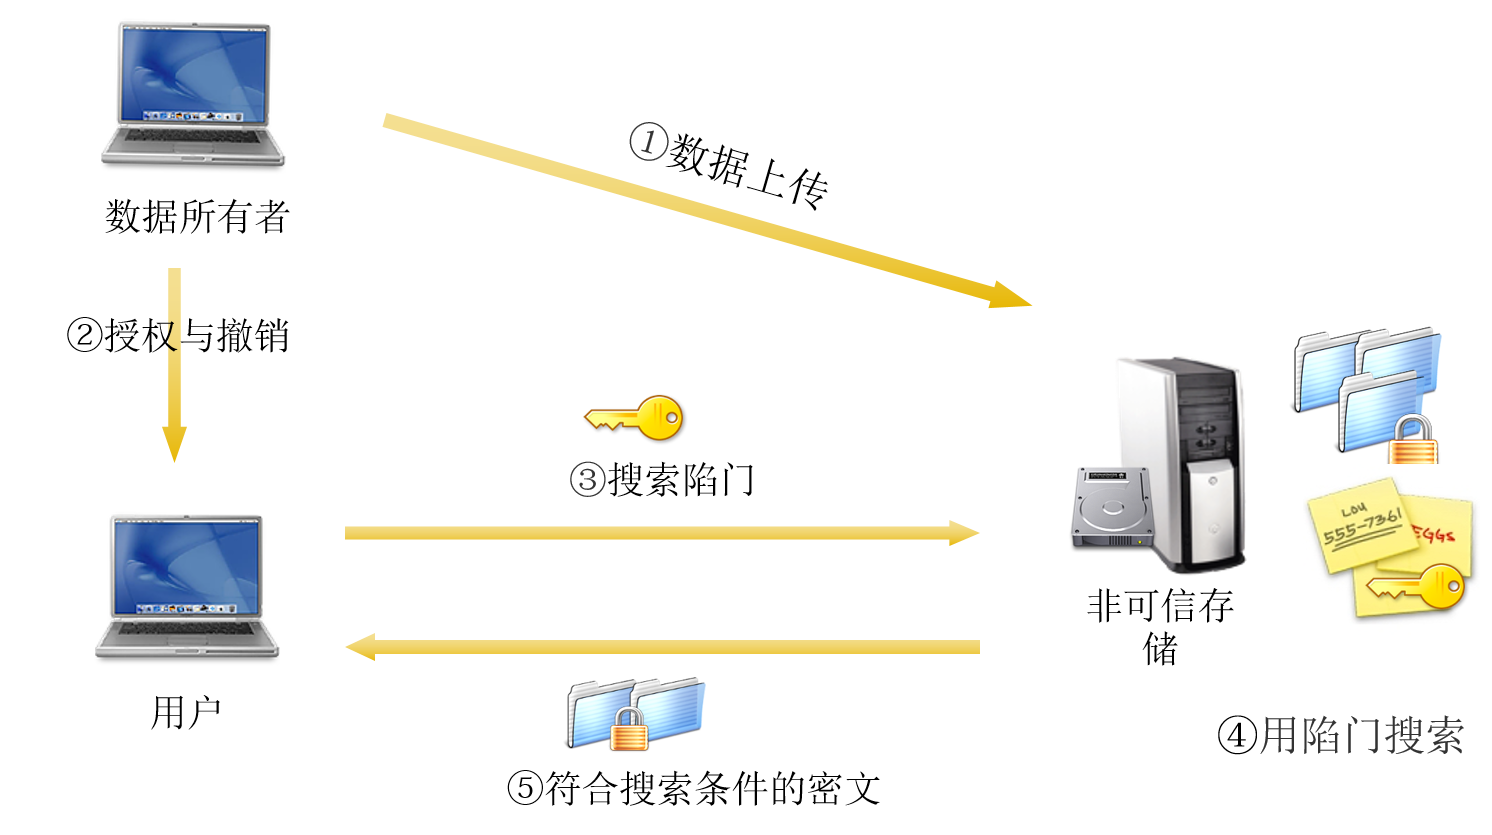
\includegraphics[width=0.9\textwidth]{chap3/general_system_model}
  \bicaption[fig:general_system_model]{对称可搜索加密的系统模型}{对称可搜索加密的系统模型}
  {Fig}{A General System Model in SSE}
\end{figure}


从图\ref{fig:general_system_model}可知,一个典型的模型有三部分组成:数据所有者、授权用户和非可信服务器。
通常数据所有者拥有数据,一个被授权的组织可以对加密的数据进行查找。过程如下:数据拥有者上传待外包的文档
并维护对加密数据的高效检索,并且对某个组织内的所有用户进行授权或撤销;被授权的用户可随时对远程加密的数据
进行搜索,并对接收的结果解密;服务器具有对加密数据进行各种条件搜索的能力,并返回符合条件的答案。我们对
数据所有者给用户进行授权和撤销的细节没有考虑,可以使用各种技术完成(公钥加密或私钥加密等) --- 仅仅传递密钥,
信息量小。



针对该系统模型,这里简单介绍一个具有代表性的基于inverted-index的对称可搜索加密方案,
该方案由五个算法组成:$SSE = (Gen, Enc, Trpdr, Search, Dec)$,数学定义如下:
\begin{enumerate}
  \item
  $Gen(1^k ) \rightarrow K$:给定安全参数$k$,生成密钥$K$;

  \item
  $Enc(K,D) \rightarrow (I,c)$:给定一组文档$D={D_1,D_2  ,…D_n  }$,使用密钥$K$加密,
  生成安全索引$I$和密文文档集合$c =\{c_1, c_2, ..., c_n \}$;


  \item
  $Trpdr(K,w) \rightarrow t_w$:给定一个单词$w$,使用密钥$K$调用陷门生成函数,输出对应的陷门$t_w$;

  \item
  $Search(I,t_w) \rightarrow R$:对陷门$t_w$在安全索引$I$上进行搜索,输出所有包含单词陷门的文档$ID$集合$R$;

  \item
  $Decrypt(K, c_i) \rightarrow D_i$:使用密钥$K$对文档$c_i$解密,生成$D_i$。

\end{enumerate}
数据拥有者首先调用$Gen$算法生成密钥并保存在本地,然后对需上传的文档调用$Enc$算法,
生成安全索引和一组加密文档,并上传至服务器。当需要检索时,用户调用$Trpdr$算法生成待搜索单词的陷门,
并发至服务器;然后服务器调用算法$Search$,使用收到的陷门在安全索引上查找,输出所有符合条件的文档$ID$,
并将对应的加密数据返回给请求者。最后,数据拥有者调用$Decrypt$算法解密加密文档。



%%%%%%%%%%%%%%%%%%%%%%%%%%%%%%%%%
%%
%%   安全模型
%%
%%%%%%%%%%%%%%%%%%%%%%%%%%%%%%%%%
\section{安全模型}
\label{sec:search_symm_security_model}

对称可搜索加密技术(SSE)的安全证明模型与密码学中常用的安全证明模型(通常是CPA和CCA))有所不同。
根据实际的场景,当前SSE大多以选择关键字攻击(CKA)做为安全分析模型。这里,我们选择两个具有代表性的安全级别
(Non-Adaptive安全和Adaptive安全),并分别从语义安全(semantic security)和不可区分安全
(indistinguishability security)进行描述。这里介绍的所有知识引用自curtmola的方案\cite{curtmola2006searchable}。
%%对称可搜索加密技术(SSE)中信息泄漏主要发生在搜索阶段,以单词所携带的信息量为单位,我们以选择关键字
%%攻击(CKA)(不同于CPA和CCA)为攻击模型进行安全分析。%为此,正式的定义安全模型之前,首先定义一些基本概念。


%%%%%%%%%%%%%%%%%%%%%%%%%%%%%%%%%%%%%%%%%%%%%%%%%
\begin{defn}[History]
\label{defn:attack_history}

假定$\Delta$代表单词词典,$D$表示在字典$\Delta$上的一组文档集合。
$D$上$q$次查询的历史(History) 定义为一个元组$H = (D,w)$,
其中$w$是包含$q$个单词的集合:$w = (w_1,...,w_q)$。

\end{defn}
%%%%%%%%%%%%%%%%%%%%%%%%%%%%%%%%%%%%%%%%%%%%%%%%%


%%%%%%%%%%%%%%%%%%%%%%%%%%%%%%%%%%%%%%%%%%%%%%%%%
\begin{defn}[Access Pattern]
\label{defn:attack_access_pattern}
假定$\Delta$代表单词词典,$D$表示在字典$\Delta$上的一组文档集合。
$D$上$q$次查询历史$H = (D,w)$的访问模式(Access Pattern)定义为一个元组 $ \partial (H)=(D(w_1 ),…,D(w_q))$。
\end{defn}
%%%%%%%%%%%%%%%%%%%%%%%%%%%%%%%%%%%%%%%%%%%%%%%%%



%%%%%%%%%%%%%%%%%%%%%%%%%%%%%%%%%%%%%%%%%%%%%%%%%
\begin{defn}[Search Pattern]
\label{defn:attack_search_pattern}
假定$\Delta$代表单词词典,$D$表示在字典$\Delta$上的一组文档集合。$D$上$q$次查询历史 $H=(D,w)$的搜索模式(Search Pattern)定义为对称二元矩阵$ \sigma(H) = \left(
  \begin{array}{cccc}
     x_{1,1} & x_{1,2} & ... & x_{1,q}  \\
    . & . & ... & . \\
    . & . & ... & . \\
     x_{q,1} & x_{q,1} & ... & x_{q,q}  \\
  \end{array}
\right)$ 。对于任意$1 \leq i,j \leq q$,如果$w_i = w_j$,则$x_{i,j}$为1,否则为0。
\end{defn}
%%%%%%%%%%%%%%%%%%%%%%%%%%%%%%%%%%%%%%%%%%%%%%%%%

%%%%%%%%%%%%%%%%%%%%%%%%%%%%%%%%%%%%%%%%%%%%%%%%%
\begin{defn}[Trace]
\label{defn:attack_trace}
假定$\Delta$代表单词词典,$D$表示在字典$\Delta$上的一组文档集合。$D$上$q$次查询历史 $H = (D,w)$的Trace定义为:$τ(H)=(|D_1 |,...,|D_n |,\partial(H),\sigma(H))$,其中$|D_i |(1 \leq i \leq n)$代表第$i$ 个文档的长度。
\end{defn}
%%%%%%%%%%%%%%%%%%%%%%%%%%%%%%%%%%%%%%%%%%%%%%%%%


\begin{defn}[Non-singular history]
\label{defn:attack_non_singular_history}
如果对任意的历史$H$满足:(1)至少存在一个历史 $H' \neq H$,使$\tau(H') = \tau(H)$;(2)在给定的$\tau(H)$ 下,历史$H'$可以在多项式时间内被发现;则称历史$H$是Non-singular。
\end{defn}
%%%%%%%%%%%%%%%%%%%%%%%%%%%%%%%%%%%%%%%%%%%%%%%%%



下面我们分别给出了在对称可搜索加密环境下的Non-adaptive和Adaptive的安全模型,
如图\ref{fig:non_or_adaptive} 所示,然后给出相关的定义。

\begin{figure}[!htp]
  \centering
  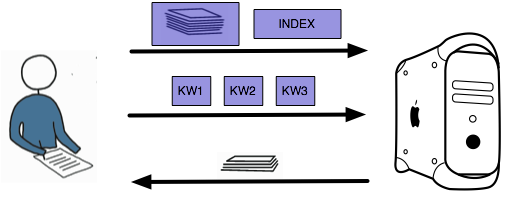
\includegraphics[width=0.45\textwidth]{chap2/non_adaptive}
  \hspace{1cm}
  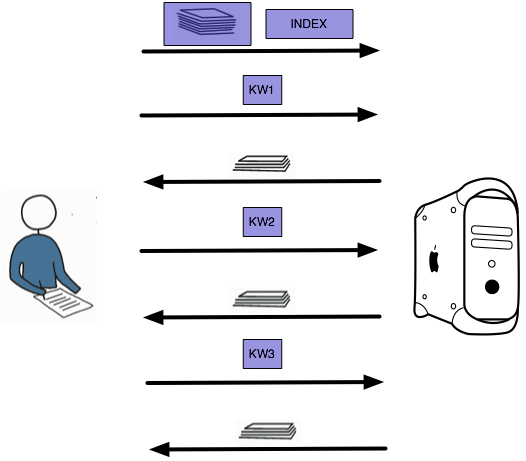
\includegraphics[width=0.45\textwidth]{chap2/adaptive}
  \bicaption[fig:non_or_adaptive]{SSE上Non-adaptive和Adaptive安全模型}{SSE上Non-adaptive和Adaptive安全模型}{Fig}{The Security Model of Non-adaptive and Adaptive in SSE}
\end{figure}



\subsection{\textbf{Non-Adaptive安全模型}}
\label{sec:search_symm_security_model_nonadaptive}

%%
%% definition 2.13
%%
\begin{defn}[Non-adaptive Indistinguishability]
\label{defn:non_adaptive_indistinguishability}
在词典为$\Delta$,安全参数为$k \in \mathbb{N}$的基础上,设$SSE = (Gen, Enc, Trpdr, Search,Dec)$是一个基于安全索引的对称可搜索加密方案,
且$\mathcal{A}=(\mathcal{A}_1,\mathcal{A}_2)$为$non-uniform$的敌手,考虑下面的概率试验${\textbf{Ind}}_{(SSE,\mathcal{A})}(k)$:
\begin{center}
\begin{tabular}{ l  }
    $\textbf{Ind}_{SSE,\mathcal{A}}(k)$                           \\
    \quad $K \leftarrow Gen(1^k)$                       \\
    \quad $(st_\mathcal{A},H_0,H_1) \leftarrow \mathcal{A}_1(1^k)$          \\
    \quad $ b \overset{\$}{\leftarrow} {0,1}$           \\
    \quad parse $H_b$ as $(D_b,w_b)$                    \\
    \quad $(I_b,c_b) \leftarrow Enc_K(D_b)$             \\
    \quad $for 1 \leq i \leq q $                        \\
    \quad \quad $t_{b,i} \leftarrow Trpdr_K(w_{b,i})$   \\
    \quad let $t_b = (t_{b,1}, ..., t_{b,q})$           \\
    \quad $b' \leftarrow \mathcal{A}_2(st_\mathcal{A},I_b,c_b,t_b)$         \\
    \quad if $b' = b$, output 1                         \\
    \quad otherwise output 0
\end{tabular}
\end{center}
假设在$\tau(H_0) = \tau(H_1)$,$st_\mathcal{A}$ --- 表示敌手$\mathcal{A}$的状态信息的前提下,如果对于任意多项式的敌手$\mathcal{A}$,有:
\begin{center}
$Pr[\textbf{Ind}_{SSE,\mathcal{A}}(k) = 1] \leq \frac{1}{2} + negl(k)$,\\
\end{center}
则称该SSE方案在Non-adaptive不可区分的条件下是安全的。
\end{defn}



%%
%% definition 2.14
%%
\begin{defn}[Non-adaptive Semantic Security]
\label{defn:non_adaptive_semantic_security}
在词典为$\Delta$,安全参数为$k \in \mathbb{N}$基础上,设$SSE = (Gen, Enc, Trpdr, Search, Dec) $是一个基于安全索引的对称可搜索加密方案,$\mathcal{A}$为一个敌手,$\mathcal{S}$是一个模拟器(Simulator),考虑下面概率过程:
\begin{center}
\begin{tabular}{ l l }
    $\textbf{Real}_{SSE,\mathcal{A}}(k)$  &  $\textbf{Sim}_{SSE,\mathcal{A},\mathcal{S}}$    \\
    \quad $K \leftarrow Gen(1^k)$   &   \quad $(H,st_\mathcal{A}) \leftarrow \mathcal{A}(1^k)$ \\
    \quad $(st_\mathcal{A},H) \leftarrow \mathcal{A}(1^k)$ & \quad $V \leftarrow S(\tau (H))$ \\
    \quad parse $H$ as $(D,w)$          &   \quad output $V$ and $st_\mathcal{A}$             \\
    \quad $(I,c) \leftarrow Enc_K(D)$            &   \\
    \quad for $1 \leq i \leq q $                 &   \\
    \quad \quad $t_i \leftarrow Trpdr_K(w_i)$    &   \\
    \quad let $t = (t_i, ..., t_q)$              &    \\
    \quad output $V = (I,c,t)$ and $st_\mathcal{A}$    &
\end{tabular}
\end{center}
如果对于任何多项式规模敌手$\mathcal{A}$,都存在一个模拟器$\mathcal{S}$,使得对于任意多项式规模的区分器$\mathcal{D}$,有:
\begin{center}
$|Pr[\mathcal{D}(V,st_\mathcal{A})] = 1 : (V,st_\mathcal{A}) \leftarrow \textbf{Real}_{SSE,A}(k)] - Pr[\mathcal{D}(v,st_\mathcal{A})=1 : (V,st_\mathcal{A} \leftarrow \textbf{Sim}_{SSE,\mathcal{A},\mathcal{S}}(k)] | \leq negl(k)$,
\end{center}
则称该SSE在Non-adaptive的条件下是语义安全的。
\end{defn}




%%%%%%%%%%%%%%%%%%%%%%%%%%%%%%%%%%%%%%%%%
%%
%%
%%     Adaptive安全模型
%%
%%
%%%%%%%%%%%%%%%%%%%%%%%%%%%%%%%%%%%%%%%%%
\subsection{\textbf{Adaptive安全模型}}
\label{sec:search_symm_security_model_adaptive}

%%
%% definition 2.15
%%
\begin{defn}[Adaptive Indistinguishability]
\label{defn:adaptive_indistinguishability}
在词典为$\Delta$,安全参数为$k \in \mathbb{N}$的基础上,设$SSE = (Gen, Enc, Trpdr, Search,Dec)$是一个基于安全索引的对称可搜索加密方案,且$ \mathcal{A}=(\mathcal{A}_1, ...,\mathcal{A}_{q+1})$为$non-uniform$ 的敌手,考虑下面的概率试验${\textbf{Ind}}^{*}_{(SSE,\mathcal{A})}(k)$:
\begin{center}
\begin{tabular}{ l  }
    $\textbf{Ind}^{*}_{SSE,\mathcal{A}}(k)$                           \\
    \quad $K \leftarrow Gen(1^k)$                       \\
    \quad $ b \overset{\$}{\leftarrow} {0,1}$           \\
    \quad $(st_\mathcal{A},D_0,D_1) \leftarrow \mathcal{A}_0(1^k)$          \\
    \quad $(I_b,c_b) \leftarrow Enc_K(D_b)$    \\
    \quad $(st_A, w_{0,1}, w_{1,1}) \leftarrow \mathcal{A}_1(st_\mathcal{A},I_b)$ \\
    \quad $t_{b,1} \leftarrow Trpdr_K(w_{b,1}) $   \\
    \quad for $2 \leq i \leq q,$ \\
    \quad \quad $(st_\mathcal{A},w_{0,i}, w_{1,i} \leftarrow \mathcal{A}_i(st_\mathcal{A},I_b,c_b,t_{b,1}, ..., t_{b,i-1}) $ \\
    \quad \quad  $t_{b,i} \leftarrow Trpdr_K(W_{b,i}) $ \\
    \quad let $t_b = (t_{b,1}, ..., t_{b,q})$           \\
    \quad $b' \leftarrow \mathcal{A}_{q+1}(st_\mathcal{A},I_b,c_b,t_b)$     \\
    \quad if $b' = b$, output 1                         \\
    \quad otherwise output 0
\end{tabular}
\end{center}
在$\tau (D_0,w_{0,1}, ..., w_{0,q}) = \tau(D_1,w_{1,1}, ..., w_{1,q})$的前提下。如果对于所有多项式规模的敌手$\mathcal{A} =(\mathcal{A}_0, ..., \mathcal{A}_{q+1})$,均有有:
\begin{center}
$Pr[\textbf{Ind}^{*}_{SSE,\mathcal{A}}(k) = 1] \leq \frac{1}{2} + negl(k)$,\\
\end{center}
则称该SSE方案在adaptive不可区分的条件下是安全的。
\end{defn}

%%
%% definition 2.16
%%
\begin{defn}[Adaptive Semantic Security]
\label{defn:adaptive_semantic_security}
在词典为$\Delta$,安全参数为$k \in \mathbb{N}$基础上,设$SSE = (Gen, Enc, Trpdr, Search, Dec)$是一个基于安全索引的对称可搜索加密方案,$\mathcal{A} = (\mathcal{A}_0, ..., \mathcal{A}_q)$为敌手,$\mathcal{S} = (\mathcal{S}, ..., \mathcal{S}_q)$是模拟器(Simulator),考虑下面概率过程:
\begin{center}
\begin{tabular}{ l l }
    $\textbf{Real}^{*}_{SSE,\mathcal{A}}(k)$  &  $\textbf{Sim}^{*}_{SSE,\mathcal{A},\mathcal{S}}$    \\
    \quad $K \leftarrow Gen(1^k)$   &   \quad $(D,st_\mathcal{A}) \leftarrow \mathcal{A}_0(1^k)$ \\
    \quad $(D,st_\mathcal{A}) \leftarrow \mathcal{A}_0(1^k)$ & \quad $(I,c,st_\mathcal{S}) \leftarrow \mathcal{S}_0(\tau(D))$ \\
    \quad $(I,c) \leftarrow Enc_K(D)$  &  \quad $(w_1,st_\mathcal{A} \leftarrow \mathcal{A}_1(st_\mathcal{A},I,c)$ \\
    \quad $(w_1, st_\mathcal{A}) \leftarrow \mathcal{A}_1(st_\mathcal{A},I,c)$ & \quad $(t_1,st_\mathcal{S}) \leftarrow \mathcal{S}_1(st_\mathcal{S}, \tau(D,w_1))$ \\
    \quad $t_1 \leftarrow Trpdr_K(w_1)$   & \quad for $ 2 \leq i \leq q$  \\
    \quad for $2 \leq i \leq q $         &  \quad \quad $(w_i,st_\mathcal{A}) \leftarrow \mathcal{A}_i(st_\mathcal{A},I,c,t_1, ..., t_{i-1})$      \\
    \quad \quad $(w_i,st_\mathcal{A}) \leftarrow \mathcal{A}_i(st_\mathcal{A},I,c,t_1, ..., t_{i-1})$    &   \quad \quad $(t_i,st_\mathcal{S}) \leftarrow \mathcal(S)_i(st_\mathcal{S}, \tau(D,w_1, ..., w_i))$  \\
    \quad \quad $t_i \leftarrow Trpdr_K(w_i)$    & \quad let $t = (t_1, ..., t_q)$  \\
    \quad let $t = (t_1, ..., t_q)$              &   \quad output $V = (I,c,t)$ and $st_\mathcal{A}$ \\
    \quad output $V = (I,c,t)$ and $st_\mathcal{A}$    &
\end{tabular}
\end{center}
如果对于任何多项式规模敌手$\mathcal{A} = (\mathcal{A}_0, ..., \mathcal{A}_q)$,都存在模拟器$\mathcal{S} = (\mathcal{S}, ..., \mathcal{S}_q)$,使得对于任意多项式规模的区分器$\mathcal{D}$,有:
\begin{center}
$|Pr[\mathcal{D}(V,st_\mathcal{A})] = 1 : (V,st_\mathcal{A}) \leftarrow \textbf{Real}^*_{SSE,A}(k)] - Pr[\mathcal{D}(v,st_\mathcal{A})=1 : (V,st_\mathcal{A}) \leftarrow \textbf{Sim}^*_{SSE,\mathcal{A},\mathcal{S}}(k)] | \leq negl(k)$,
\end{center}
则称该SSE在adaptive的条件下是语义安全的。
\end{defn}

Curtmola在论文\cite{curtmola2006searchable}中分别证明Non-adaptive不可区分安全性与Non-adaptive语义安全和adaptive不可区分安全性与adaptive语义安全是等价的。


%%%%%%%%%%%%%%%%%%%%%%%%%%%%%%%%%%%%%%%%%%%%%%%%%%%%%
%%
%%      对称可搜索加密技术
%%
%%%%%%%%%%%%%%%%%%%%%%%%%%%%%%%%%%%%%%%%%%%%%%%%%%%%%
\section{对称可搜索加密方案分类}
\label{sec:search_symm_symm}


%%%%%%%%%%%%%%%%%%%%%%%%%%%%%%%%%%
%%
%%  单关键字搜索
%%
%%%%%%%%%%%%%%%%%%%%%%%%%%%%%%%%%%
\subsection{单关键字搜索}
\label{sec:search_symm_symm_exact}

对于可搜索加密问题,Goh在文章\cite{goh2003secure}中的提出了第一个基于正向索引的解决方案。
方案使用一个Bloom Filter\cite{gremillion1982designing}作为安全索引。
对于每个文档,映射包含的所有单词到一个Bloom Filter;在搜索时,授权用户发送待查单词的多个哈希
值作为陷门;一旦服务器收到请求后,逐个检查每个Bloom Filter,判断对用的位置是否是“1”,
如果全部都为“1”,则表示包含该单词并返回该文档,否则跳过。该方案突出的优势体现在性能上:
Bloom Filter的映射过程只需要计算若干Hash函数,故索引创建过程性能较高。在搜索阶段,
服务器需要对每个文档调用一次SearchIndex算法,而在该算法中对陷门中每个元素只需进行Bloom
Filter数据位的比较操作,时间复杂度仅为$O(1)$,故整体效率仍然是比较高的。但是该方案却引进了误报率,
且误报率和安全索引的大小成反比关系。

Y. Chang在\cite{chang2005privacy}中则基于forward-index提出了没有误报率的的方案。其基本思想如下:
将待上传文档中所有出现的单词构成一个词典,安全索引中用一比特位代表每个单词是否存在
--- “1”表示存在该单词,“0”表示不存在。方案同样达到了相当高的效率,但问题在于词典的保存大大增加
了存储开销的负担。文中给出了两个解决方案,第一个方案是将词典保存在客户端,这样用户每次查询则
需要本地词典,这样增加了本地的存储和计算开销,并且在多用户环境下还需要同步词典;第二个方案则
将词典加密后存放在远程服务器上,但查询过程则需要通讯两轮 --- 一轮获得词典里索引信息,另一轮查询
获得文档。

R.Curtmola在文章\cite{curtmola2006searchable}中第一次基于inverted-index给出了两个改进方案,
并给出了详细的安全性定义和证明。第一个方案达到了Non-adaptive安全性,其基本思想描述如下:
首先构建待上传文档的inverted-index;然后将索引表项中的文档ID部分加密并随机分散到一个数组中,
如下图\ref{fig:curtmolaInvertedIndex}所示:

\begin{figure}[!htp]
  \centering
  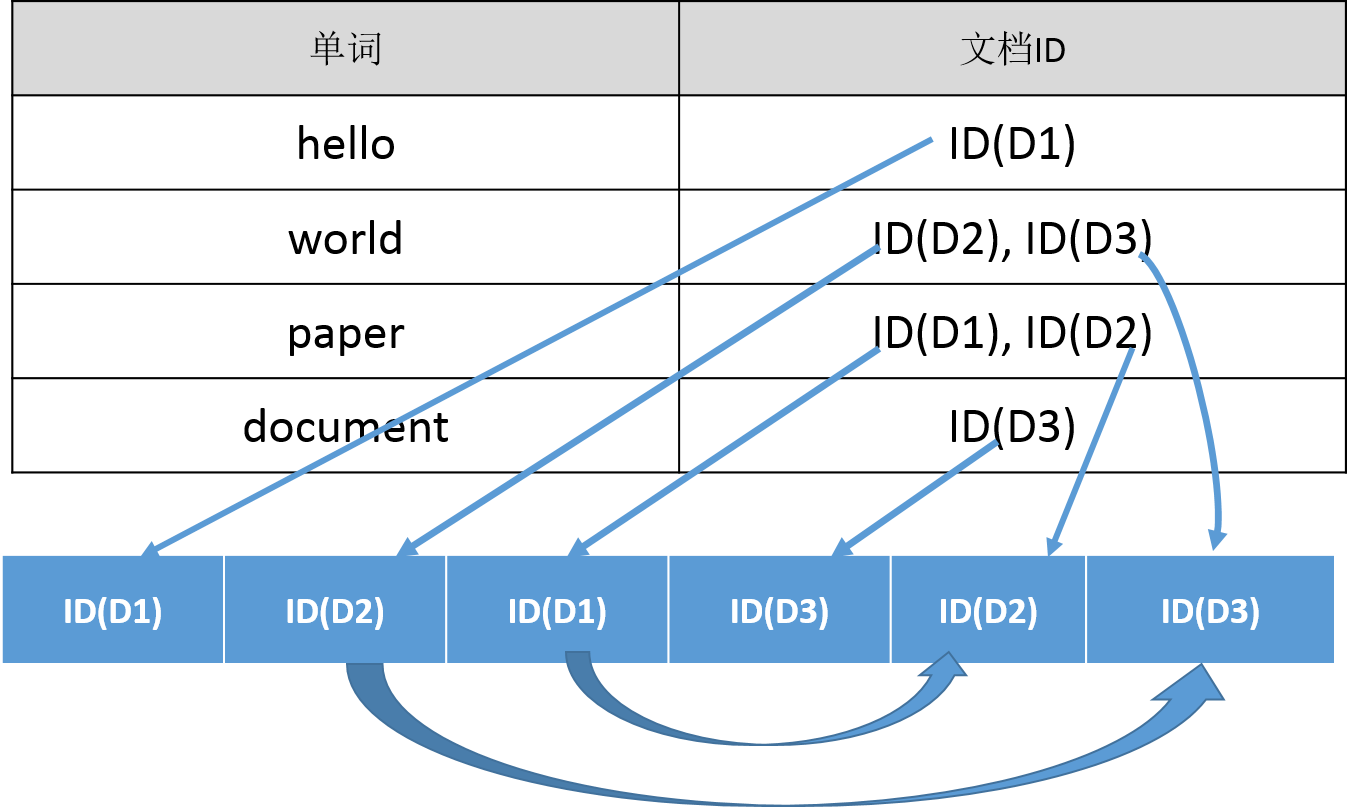
\includegraphics[width=0.8\textwidth]{chap2/curtmolaInvertedIndex}
  \bicaption[fig:curtmolaInvertedIndex]{文档ID数组}{文档ID数组}{Fig}{The Array of Document ID}
\end{figure}

从上表可知,每个单词所对应文档的ID形成一个链表。数组中的每个元素使用不同的密钥调用对称分组密码算法加密。而文档中所有的单词在Inverted-index则以查找表的形式存储,如图\ref{fig:curtmolaSearchTable} 所示:
\begin{figure}[!htp]
  \centering
  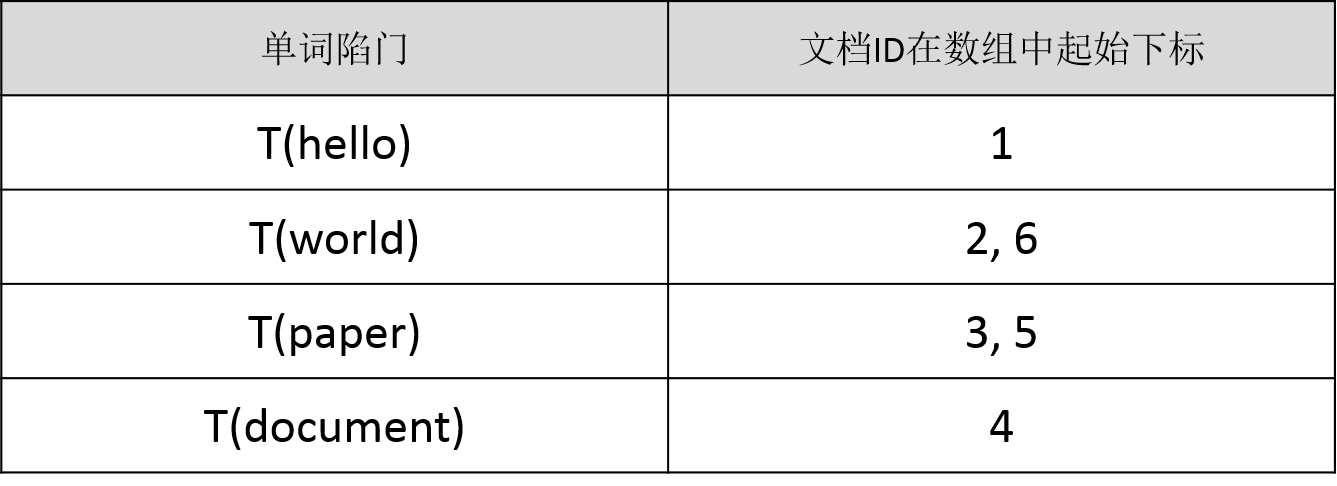
\includegraphics[width=0.8\textwidth]{chap2/curtmolaSearchTable}
  \bicaption[fig:curtmolaSearchTable]{反向安全索引中的查找表}{反向安全索引中的查找表}{Fig}{The Look-up Table of Secure Index}
\end{figure}


查找表的条目由键值对的形式表示,其键存储的是通过伪随机函数对单词置换后的结果 --- 单词的陷门,
其值所存储的部分为对应文档$ID$的链表在数组中的起始位置。
查找的时候,通过单词的陷门在查找表处找到其$ID$链表在数组中的起始位置,
然后根据起始$ID$位置逐个解密这个链表获得所有包含该单词的文档$ID$集。

Curtmola方案一的主要优势是服务器端的搜索效率高,得益于inverted-index,其服务器端搜索时间复杂度为$O(1)$,
而之前的方案都只能达到$O(n)$($n$表示文档的数目)。同时R. Curtmola在文中给出了另一个具有
Adaptive安全性的方案,服务器端搜索时间复杂度仍能保持$O(1)$,但是服务器端的存储量和单词陷门的大小均有所增加。

为了确保方案足够安全 --- 不能因$ID$链表元素个数不同而导致信息泄漏,Curtmola建议数组元素的个数应与
所有文档的总长度所能容纳的最大单词数相当。这将导致在安全索引中,数组部分所占用的存储空间将会远大于
所有文档的总长度。H. Lu在文章\cite{jin2012reducing}中基于inverted-index提出了一种降低安全索引
结构所占存储空间的方案。方案与Curtmola在方案1的最大不同在于合并了安全索引中$ID$链表结构中相同的
元素,从而极大减少了数组的长度,如图\ref{fig:luInvertedIndex}所示:
\begin{figure}[!htp]
  \centering
  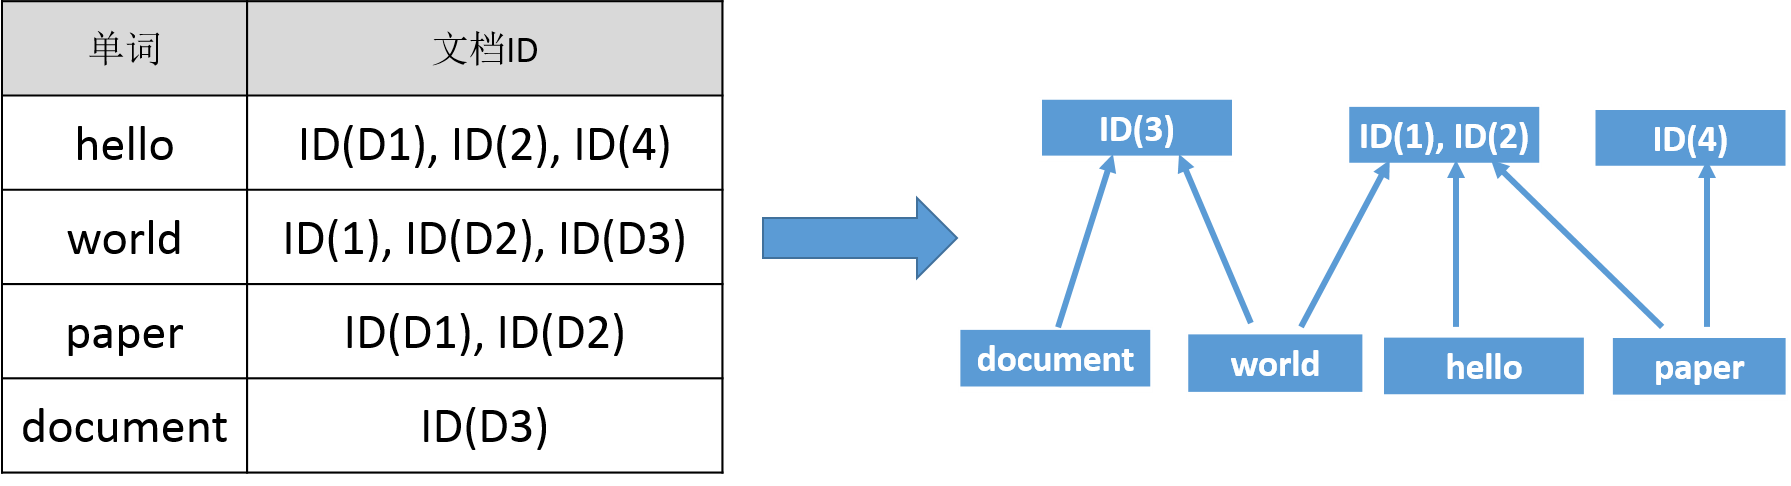
\includegraphics[width=0.8\textwidth]{chap2/luInvertedIndex}
  \bicaption[fig:luInvertedIndex]{改进的文档ID链表}{改进的文档ID链表}{Fig}{An Improved List of Documents ID}
\end{figure}

基于这样的结构使得合并后每个文档$ID$在数组中只出现一次,从而减少数组元素的总数。经实际测试,
方案中数组的元素个数可降至原来的5\%以下。

作者Van在\cite{van2010computationally}中基于inverted-index提出了另一种形式的安全索引方案,
方案使用一个加密的二元数组维护安全索引信息,数组两维分别表示单词和文档$ID$,数组元素为“1”表示对应
的文档包含对应的单词。搜索时解密二维数组中对应单词所在的行,即可知晓包含该单词的文档$ID$。



\subsection{模糊搜索}
\label{sec:search_symm_symm_fuzzy}

在加密的云数据环境中,当前的相似搜索的研究集中在模糊搜索上。基于明文模糊搜索\cite{ji2009efficient}
\cite{li2008efficient} \cite{behm2009space} 和精确关键字搜索\cite{curtmola2006searchable}
\cite{chang2005privacy} \cite{jin2012reducing},Jin Li等人于2010年在\cite{li2010fuzzy}中率先提出了
模糊对称可搜索加密的问题,并提供了两种解决方案:直接模糊搜索方案和基于通配符的模糊搜索方案。方案用
编辑距离(edit distance\cite{ristad1998learning})来衡量单词之间的相似性,即若给定单词$w_1$和$w_2$,
定义其编辑距离为:将$w_1$变换成$w_2$所需的最小的操作数,变换操作包括:(1)插入:在单词的某个位置上
插入一个字符;(2)删除:删除单词中某个字符;(3)替换:将单词中某个字符替换为另一个字符。该方案的基
本思想如下:(1)加密阶段:对文档集中每个单词$w$构建模糊集$F_w$,用与\cite{curtmola2006searchable}方
案相同方式构建反向安全索引,然后将安全索引和加密文档外包;(2)陷门生成阶段:当搜索单词$w$时,首先构
建单词$w$的模糊集$F_w$,然后计算集合$F_w$所有单词的陷门并提交至服务器;(3)搜索阶段:当服务器收到请
求的陷门后,在安全索引中查询是否存在和单词$w$的陷门精确匹配的索引,若存在则返回,否则返回与模糊集
$F_w$所有陷门匹配的结果。

在直接的模糊搜索方案中,构建单词$w$的模糊集如下:枚举所有的单词$w'$使得$ed(w,w') \leq d$。
而在改进的模糊搜索方案中,用通配符来替代同一位置上所有不同的单词,这样大大降低了模糊集的规模,
降低了网络传输开销和服务端的存储开销。但是不幸的是,方案对服务器存储开销与编辑距离正相关,
且不支持多关键字搜索。同时,不同单词的模糊集之间存在碰撞,例如当单词$“at”$ 和$“it”$ 在编辑距离为1时,
对应模糊集分别为:$S_{at,1}=\{*at,*t,a*t,a*,at*\}$, $S_{it,1}= \{*it,*t,i*t,i*,it* \}$($S_{w,d}$
表示单词$w$在编辑距离为$d$时的模糊集),有$S_{at,1} \cap  S_{it,1} \neq \varnothing $。

为了解决上述方案中服务端存储过大的问题,M. Chuah等人在\cite{chuah2011privacy}中提出了基于
BedTree\cite{zhang2010bed}的模糊可搜索加密方案。方案的具体过程如下:(1)加密阶段:对于单
词$w$在编辑距离为$d$时,将其模糊集对应的陷门映射到Bloom Filter中,
如将$S_{w,i}$ 映射到$B_i$中($S_{w,i}$ 表示单词$w$在编辑距离为$i$时的模糊集,
$B_i$表示编辑距离为$i$时模糊集所构造的Bloom Filter),然后将单词的$ \{B_i, i \leq d \}$、
单词所对应文档的ID信息以及单词的陷门作为一个叶子节点,通过单词的数据向量插入到BedTree树中;
(2)陷门生成阶段:对待搜索单词$w$,计算其数据向量和模糊集中每个元素的陷门,并提交至服务端;
(3)搜索阶段:当服务器收到用户的查询信息后,首先通过其数据向量在BedTree树构造的安全索引中
查找某叶子节点,再检查模糊集陷门是否存在于$B_i$中,最终返回正确匹配的结果集。该方案主要在安全
索引结构上有所改进,利用BedTree的索引结构降低了存储空间和Bloom Filter减少了索引构建时间,
同时能很好地扩展到多关键词搜索和增量更新。然而,方案也引入了新的的问题 --- 由Bloom Filter引入
了一定的误报率。

Cong Wang等人在\cite{wang2012achieving}中基于Trie树的结构提出了搜索效率更高且具备同等安全的模糊可
搜索加密方案。他们首先对方案\cite{li2010fuzzy}提出了改进措施:对每个单词$w$,根据容许的最大编辑距离
$d$计算出单词的模糊集$S_{w,d}$,然后根据Bloom Filter技术将每个单词的模糊集计算出的令牌映射到一个
Bloom Filter,即对每个关键字的模糊集构建一个Bloom Filter;在搜索关键字$w$时,
服务端只需搜索待搜索单词模糊集对应令牌是否存在某个Bloom Filter中,即可查询得到所需的结果。
基于\cite{li2010fuzzy}的改进方案虽然减少服务器的存储量,但是却增加了服务端的搜索时间 ---
对所有关键字构建的Bloom Filter索引都要搜索一次,并且由Bloom Filter结构带来了一定的误报率。
方案的构建过程如下:(1)加密阶段:首先计算文档中每个单词的模糊集和对应令牌信息。然后对于每个令牌将其分成N块,并将N块的子结构插入到Trie 树中,叶子节点即单词令牌的最后一块,并将单词对应文档信息放在叶子节点中或者在当前叶子节点下插入一个新的节点存放其他信息,最后将安全索引和文档密文外包到服务端;(2)陷门生成阶段:对单词$w$,计算模糊集及对应令牌,并发送给服务端;(3)搜索阶段:当服务端收到用户发来的令牌集后,首先对单词$w$的令牌按照构建索引过程分成N块,然后在基于Trie树的索引中进行精确查找,若找到返回精确查询的结果,否则对其模糊集令牌按照同样方式搜索并返回结果集。该方案主要基于不同单词之间存在相同的部分,通过相同的部分来减少存储量。该方案与方案\cite{li2010fuzzy}相比,明显减少了服务端的存储开销但是增加了常量的搜索时间。与方案\cite{chuah2011privacy}相比,该方案减少了搜索过程中信息的泄漏增强了方案的安全性,但是从数据的时间局部性和空间局部性的角度来看,由于BedTree是一颗B+树,而Trie是一棵多叉树,因而B+树可以利用数据局部性原理来通过减少内存在访问过程中搜索失效时数据内存时间换入换出来提高单词的搜索时间。

Deshpande等人在\cite{balamuralikrishna2013fuzzy}中对目前所有模糊可搜索加密方案进行了总结 --- 包括
一般的基于通配符构建模糊集的可搜索加密方案、基于BedTree树构建索引的模糊可搜索加密方案和基于Trie树
构建索引的模糊可搜索加密方案;并提出了两种高效的模糊单词集构建方案 --- 基于通配符和Gram;并通过实
验分析了各方案在不同编辑距离时索引构建的时间和搜索的时间及个方案相关优缺点。

上述方案都以编辑距离来衡量单词间的模糊程度,不可避免带来了碰撞,引入了安全隐患。为此,
\cite{boldyreva2014efficient}第一次提出了sub-linear的模糊可搜索加密方案。在方案中,
他们使用了基于有权图的理论来描述单词间的相似性,并对此提出了一个更强的安全定义,
证明之前方案并不能达到此安全。此外,他们也给出了如何在安全性和高效性做出平衡。

\subsection{动态搜索}
\label{sec:search_symm_symm_dynamic}

基于正向索引的解决方案\cite{goh2003secure} \cite{chang2005privacy}等都能很好地适应与动态的搜索领域。
对于扩展于动态搜索,索引结构的调整非常简单,仅需要在正向索引中添加或删除对应条目即可。但是正向索引
的方案在查找上效率并不高,通常与文档数目相关。

为了解决上述方案中的不使用问题,Kamara等人于2012年在\cite{kamara2012dynamic}中第一次提出了
动态可搜索加密技术的问题及相应的解决方案。在文中作者主要结合了正向索引具有的动态修改特性和
反向索引的强安全性和无误报率等特征,在反向索引方案的基础上通过增加另一个正向索引,实现了具有
动态修改的可搜索加密方案。该方案不仅获得了有效的搜索时间 --- 线性搜索时间(与文档数目成正比),
而且确保了搜索过程中的信息泄漏,具有Non-adaptive的安全性。该方案的主要思想如下:在索引构建阶段,
不但对每个单词构建了一个反向索引,而且对每篇文档构建了一个正向索引,正向索引和反向索引通过对偶
节点(dual node)联系起来(所谓对偶节点即将正向索引结构中的<文档,单词>条目和反向索引结构中的<单词,文档>条目具有相同值的那对节点称为对偶节点);在搜索时,只需要查询反向安全索引即可;而在添加或删除文档时,需通过一系列复杂的位操作对正向索引和方向索引进行更新,同时维护正向索引与反向索引之间的对应关系。随后,Kamara在文章\cite{kamara2013parallel}中对\cite{kamara2012dynamic}方案进行扩展,提出具有并行特征的动态可搜索加密方案,这样可充分利用基于多核和分布式的计算机来提升方案的整体性能。但是服务器端额外存储量增加了1倍以上。

Stefanov等人在\cite{stefanov2013practical}中提出了具有更少信息泄漏和更高效的动态可搜索加密方案。
他们指出Kamara方案中泄漏的信息并不仅仅限于他们方案中所定义的信息 ---
泄漏搜索模式(search pattern)\cite{liu2014search}、
访问模式(access pattern)\cite{islam2012access}和大小模式(size pattern),
同时也存在forward privacy(即在搜索单词$w$后,然后立即添加一个包含$w$的文档,
服务器不应该了解到新添加的文档包含用户刚搜索过的单词$w$)和backward privacy
(即当删除包含某单词$w$的文档后,随之搜索单词$w$,服务器不应该了解到刚被删除的文档包含单词$w$)
的信息泄漏。作者在文中第一次提出具有forward privacy安全的动态可搜索加密方案,
但是backward privacy的信息泄露问题仍然没有得到解决。


\subsection{优先级搜索}
\label{sec:search__symm_symm_ranked}
支持优先级搜索的可搜索加密技术(Ranked Keyword Search)是指对于文档中出现的单词,其对应的搜索结果
文档具有不同的优先级 --- 如文档中被搜索单词出现次数多则优先级高,反之则优先级低。搜索时,
服务器按优先级先后次序返回搜索结果,或者返回指定数量的优先级最高的文档。最简单的做法将客户端预先
计算的优先级加密存放到安全索引中,搜索的时候,服务器解密搜索结果文档所对应的优先级,从而进行筛选
或排序。但A. Swaminathan在\cite{swaminathan2007confidentiality}中证实:如果服务器能直接获得优先
级值的话,在特定情况下,有可能获得明文或者搜索关键词的信息。

上述方案仅仅能将结果返回给用户,不能对结果进行过滤,例如搜索结果按优先级排序。C. Wang
在\cite{wang2010secure}\cite{wang2012enabling}中最先考虑了支持单个单词的优先级对称可搜索加密技术,
给出了这类方案的具体定义,并设计了一个具体的方案。方案中对文档的优先级使用保序加密
(Order Preserving Encryption)\cite{boldyreva2011order}技术进行加密;
对于不同的单词,使用不同的密钥加密优先级。使得服务器无法得到优先级的具体值,甚至无法评估不同关键词对
应搜索结果的优先级差异,从而降低了信息泄漏,使其安全性能与之前的对称可搜索加密方案相当。

N. Cao在\cite{cao2014privacy}中将优先级搜索问题扩展到多个单词的情形,
通过coordinate matching\cite{witten1999managing}综合考虑一篇文档相对于多个搜索单词的综合优先级,
并给出了具体的支持多个搜索单词的优先级搜索方案。该方案的问题在于单词词典是固定的,如果需要增加新
的单词的话,需要进行重构操作。Z. Xu在\cite{xu2012efficient}中针对这个问题作出了改进,使得新增单
词时,只需要少量调整操作;方案中还考虑了单词访问频率对优先级的影响。J. Yu则在\cite{cao2014privacy}中
做了进一步的研究,给出了安全性更强的方案。

%%%
%%%\subsection{优先级搜索}
%%%\label{sec:search__symm_symm_ranked}
%%%支持优先级搜索的可搜索加密技术(Ranked Keyword Search)是指对于文档中出现的单词,其对应的搜索结果文档具有不同的优先级——如文档中被搜索单词出现次数多则优先级高,反之则优先级低。搜索时,服务器按优先级先后次序返回搜索结果,或者返回指定数量的优先级最高的文档。最简单的做法将客户端预先计算的优先级加密存放到安全索引中,搜索的时候,服务器解密搜索结果文档所对应的优先级,从而进行筛选或排序。但A. Swaminathan在[42]中证实:如果服务器能直接获得优先级值的话,在特定情况下,有可能获得明文或者搜索关键词的信息。
%%%C. Wang在[40][41]中最先考虑了支持单个单词的优先级对称可搜索加密技术,给出了这类方案的具体定义,并设计了一个具体的方案。方案中对文档的优先级使用保序加密(Order Preserving Encryption)[45]技术进行加密;对于不同的单词,使用不同的密钥加密优先级。使得服务器无法得到优先级的具体值,甚至无法评估不同关键词对应搜索结果的优先级差异,从而降低了信息泄漏,使其安全性能与之前的对称可搜索加密方案相当。
%%%N. Cao在[46]中将优先级搜索问题扩展到多个单词的情形,通过coordinate matching[47]综合考虑一篇文档相对于多个搜索单词的综合优先级,并给出了具体的支持多个搜索单词的优先级搜索方案。该方案的问题在于单词词典是固定的,如果需要增加新的单词的话,需要进行重构操作。Z. Xu 在[48]中针对这个问题作出了改进,使得新增单词时,只需要少量调整操作;方案中还考虑了单词访问频率对优先级的影响。J. Yu则在[49]中做了进一步的研究,给出了安全性更强的方案。
%%%
%%%
%%%
%%%\subsection{布尔搜索}
%%%\label{sec:search_symm_symm_boolean}
%%%文档搜索中的布尔搜索(boolean search)是指搜索条件为多个单词通过逻辑与或非操作连接的表达式的情形。
%%%支持布尔搜索最简单的做法对搜索条件中的每个单词应用一次单个单词的搜索算法,然后构造一个横坐标为搜索条件中的单词,纵坐标为文档ID的二元矩阵:矩阵元素为1表示对应文档中包含对应的单词,反之为0。将搜索条件表达式中的单词替代为矩阵中对应的行,最后通过按位计算的方式计算该表达式,计算结果中的“1”所对应的文档就是搜索结果。如搜索条件为(computer∨encryption)∧¯commercial时,假定通过三次单个单词的搜索,得出包含computer的文档ID为(1, 2, 4),包含encryption的文档ID为(2, 4),包含commercial的文档ID 为(4, 5),构造图7 二元矩阵如图7 所示:
%%%
%%%	单词-文档ID二元矩阵范例
%%%将对应的行代入到搜索条件中并计算:(11010∨01010)∧¯00011=11000,可知文档1和2 为搜索结果。
%%%但上述做法泄漏了过多的信息——搜索表达式中每个单词单独的搜索结果。一个安全的支持布尔搜索的可搜索加密方案应使服务器只知晓搜索表达式的搜索结果,但无法从这个过程推导表达式中每个单词单独的搜索结果或其他搜索表达式的搜索结果。
%%%
%%%P. Golle在[17]中提出了最早的支持逻辑与的布尔搜索(conjunctive search)的对称可搜索加密方案。该方案为每个文档创建一个安全索引,索引中包含文档单词及其位置信息,搜索时需提供所有参与逻辑与操作的单词陷门及其对应的位置,只有单词和位置都符合的文档才会作为搜索结果。如某文档的前五个单词分别是(alice sent this email yesterday),当搜索(1, 5, alice, yesterday)(即第一个单词为alice,第五个单词为yesterday)时,该文档将成为搜索结果的一部分;当搜索(2, 5, alice, yesterday)时,则不作为搜索结果,因为位置不对。
%%%P. Golle在文中提出了两个可证明安全的方案。第一个方案基于Decision Diffie-Hellman困难问题[18]。 构建安全索引时需要对每个单词进行一次模指数运算,搜索过程中需要对每个文档进行两次模指数运算,而且陷门的长度与文档总数成正比关系。第二个方案基于双线性映射(bilinear map),可实现常数级别的陷门长度,创建安全索引的计算量也与第一个方案大致相当,但搜索过程对每个文档所需进行的双线性映射计算次数与搜索条件中所包含的单词数成正比。
%%%上述两个方案性能均较低,只适合从文档中提取少量关键词创建安全索引,支持在这些关键词上的搜索。一个可能的应用场景是支持对电子邮件关键域信息的搜索。
%%%L. Ballard在[19]中给出了两个支持逻辑与布尔搜索的改进方案。第一个方案基于Shamir的门限秘密分享方案[20],另一个方案则是基于双线性映射。这两个方案的效率比起[17]均大为提高,第二个方案虽然也基于双线性映射,但仅有服务器端需要进行双线性映射运算。上述两个方案同样在安全索引中包含文档单词及其位置信息,只有单词和位置都符合的文档才会作为搜索结果。
%%%K. Florian在[21]中给出了一种不保存单词位置的支持逻辑与布尔搜索的方案。在这种方案中,只要文档中包含搜索条件中的所有单词,就会加入到搜索结果,而不管这些单词出现在什么位置。在该方案中,创建安全索引时需要对每个单词进行模指数运算,创建陷门和搜索时需要进行双线性映射计算,其次数与搜索条件中的单词数成正比,故整体性能较低。D. Cash在[79]中给出了一种基于Oblivious Cross-Tags的布尔搜索算法,平衡性能和安全性。
%%%以上方案均在搜索时仅能支持单词的逻辑与操作。到目前为止,唯一能同时全面支持逻辑与或非布尔搜索的方案由T. Moataz在[22]中提出的。该方案先将所有文档中出现的单词转换成相互独立的矢量,然后通过Gram-Schmidt过程[23]将其转换成一组正交基,也就是每个单词映射到一个正交基上。对于每个文档,将其包含的单词所对应正交基的和——在这个线性子空间中每个维度的坐标都是1 的矢量——作为文档的安全索引。对于只包含逻辑与的搜索表达式,在表达式中所包含的单词对应的正交基张成的线性子空间中,精心选择一个各个维度值都不为0的矢量作为陷门,搜索时只需将陷门与安全索引进行内积运算,将结果为1的文档加入搜索结果中即可。T. Moataz还进一步讨论了支持逻辑或和逻辑非的做法。该方案可以达到Adaptive语义安全。
%%%上述方案在支持布尔搜索方面,功能相当全面,但仍然存在性能和客户端存储量的问题。在作者的测试中,当单词总数达到4000个时,创建正交基需要18秒,创建时间与单词总数的平方成正比。由于该正交基在生成搜索条件陷门的时候需要使用,从计算时间来看不适合临时生成,而应该一次生成永久保存在客户端,这就增加了客户端的存储量需求。另外,无论是否保存正交基,都需要在客户端保存一个单词词典。该方案的另一个问题是动态性,当需要进行文档增加和修改操作时,如果增加了新的单词,则需要进行正交基重构,之前所有文档的安全索引都将无效;用户必须自行下载所有文档,解密并重新创建安全索引,完成后重新上传。
%%%






%%%%
%%%%%%%%%%%%%%%%%%%%%%%%%%%%%%%%%%%%%%%%%%%%%%%%%%%%%%%%%
%%%%%%
%%%%%%      公钥可搜索加密技术
%%%%%%
%%%%%%%%%%%%%%%%%%%%%%%%%%%%%%%%%%%%%%%%%%%%%%%%%%%%%%%%%
%%%%\section{公钥可搜索加密技术}
%%%%\label{sec:asym}
%%%%
%%%%
%%%%\subsection{公钥可搜索加密的基本定义}
%%%%\label{sec:asym_defintion}
%%%%
%%%%D. Boneh在[52]中最早定义了公钥可搜索加密方案的模型:
%%%%一个非交互公钥可搜索加密方案包含以下多项式时间随机算法:
%%%%\begin{enumerate}
%%%%  \item
%%%%  {$ KenGen(s) $}:根据输入的安全参数s,生成公私钥对 $A_pub$,$A_priv$;
%%%%
%%%%
%%%%  \item
%%%%  {$ PEKS(A_pub,W) $}:以单词W和公钥 $A_pub$ 作为输入,生成单词W的可搜索密文S;
%%%%
%%%%
%%%%  \item
%%%%  {$ Trapdoor(A_priv,W) $}:根据私钥 $A_priv$ 和单词W,生成搜索陷门 $T_w$;
%%%%
%%%%
%%%%  \item
%%%%  {$ Test(A_pub,S,T_w) $}:根据密文S、陷门 $T_w$ 以及公钥 $A_pub$,测试陷门对应的单词与密文所加密的单词是否相当,如相等则输入“yes”,否则输出“no”。
%%%%
%%%%\end{enumerate}
%%%%	
%%%%	
%%%%数据接收者调用$KenGen$算法生成自己的公私钥对,并发布公钥。数据拥有者以接收者的公钥使用传统方法加密文档,并将文档中允许搜索的单词与接收者的公钥作为输入调用PEKS算法进行加密,然后将所有PEKS密文与加密文档一起发送至非可信服务器。数据接收者要进行搜索时,以自己的私钥和待搜索的单词作为输入调用Trapdoor算法,生成待搜索单词的陷门,并发往服务器。服务器对于发往接收者的每个文档,将陷门与文档的每个PEKS密文调用一次Test算法,如果存在某次Test结果为yes,则将该文档加入到搜索结果中。
%%%%从模型中可以看出,公钥可搜索加密方案是对单词进行加密,而不是像对称可搜索加密方案那样对文档或者文档集合进行加密。在这种模型下,无法使用索引技术进行加速,而且公钥运算本身效率较低,故公钥可搜索加密往往只支持对文档中的少量单词进行搜索,而不支持全文搜索。
%%%%
%%%%D. Boneh在[52]中也定义了公钥可搜索加密方案的安全性:
%%%%公钥可搜素加密方案应保证PEKS算法生成的密文不泄漏明文或者密钥的任何信息,除非敌手得到了对应的陷门。定义PEKS安全游戏如下:
%%%%\begin{itemize}
%%%%  \item
%%%%  挑战者运行 $KeyGen$ 算法生成公私钥对 $A_pub$,$A_priv$,并将公钥 $A_pub$ 发送给敌手;
%%%%
%%%%  \item
%%%%  敌手自由选择单词{$ W \in {\{0,1\}}^* $},并向挑战者问询对应的陷门 $T_w$;
%%%%
%%%%  \item
%%%%  在某个时间但,敌手选择两个单词 $W_0$ 和 $W_1$,发送给挑战者,限制条件是这两个单词之前敌手没有进行过陷门问询。挑战者随机选择 $b \in \{0,1\} $,并将$C = PEKS(A_pub,W_b)$;
%%%%
%%%%  \item
%%%%  敌手可以继续进行陷门问询,前提是所问询的单词不能是$W_0$或$W_1$;
%%%%
%%%%  \item
%%%%  最后,敌手输出 $b' \in \{0,1\}n$;如果 $ b' = b $,则敌手赢得游戏。
%%%%\end{itemize}
%%%%
%%%%	
%%%%定义敌手A的优势为:
%%%%$Adv_A(s)$ = $ |Pr⁡[b' = b]-1/2| $
%%%%如果对于任意多项式时间敌手A,$Adv_A(s)$ 均为一可忽略函数(negligible function),则称该公钥可搜索加密方案是语义安全的。
%%%%
%%%%公钥可搜索加密方案存在一个安全性问题:在单词明文空间已知(如所有的英文单词)的情况下,易受关键词猜测攻击[53]。攻击思路说明如下:服务器在收到接收者发来的单词陷门后,对于单词明文空间中的每个单词,调用PEKS算法进行加密(加密过程只需要接收者的公钥),并将密文与接收者的陷门一起调用Test算法,如果TEST输出为yes,就可以知晓接收者的陷门所对应的单词了。产生这个问题的原因在于PEKS和Test算法服务器都可以直接调用,不改变这个模型难以抵御这种攻击[54]。
%%%%H. S. Rhee在[55][56]中给出了一种抵御关键词猜测攻击的公钥可搜索加密方案,其基本思想是让非可信的服务器只做数据存储,而使用一个指定的可信的服务器进行关键词搜索。这种方案在搜索服务器可信的情况下,可抵御关键词猜测攻击。但在实际中,对于客户端而言,要找到这种的可信搜索服务器并不容易。Q. Tang 在[57][62]中则选择了另一种思路,数据拥有者和数据接收者通过交互来抵御关键词猜测攻击。但是在实际中,数据拥有者和数据接收者进行安全交互并不容易。
%%%%
%%%%
%%%%\subsubsection{基本模型定义}
%%%%\label{sec:asym_definition_model}
%%%%
%%%%
%%%%\subsubsection{安全性模型}
%%%%\label{sec:asym_definition_security}
%%%%
%%%%
%%%%%%%%%%%%%%%%%%%%%%%%%%%%%%%%%%%%%%%%%%%%%%%%%%%%%%%%%
%%%%%%
%%%%%%   公钥可搜索加密的方案
%%%%%%
%%%%%%%%%%%%%%%%%%%%%%%%%%%%%%%%%%%%%%%%%%%%%%%%%%%%%%%%%
%%%%\subsection{公钥可搜索加密的方案}
%%%%\label{sec:asym_solution}
%%%%
%%%%D. Boneh在[52]中设计了三种不同的公钥可搜索加密方案,分别基于双线性映射、陷门置换和Jacobi符号。并指出公钥可搜索加密方案是一个比基于身份的加密(Identity Based Encryption,缩写IBE)[58]更难的问题。在D. Boneh的模型中,要求数据接收者和服务器之间建立安全信道。这个要求在实际中有时并不容易实现,J. Baek在[59]中研究了这个问题,修改了公钥可搜索加密的模型,使其无需任何安全信道,并给出了改进模型的方案。M. Abdalla在[60]中详细研究了公钥可搜索加密方案的一致性问题,讨论了公钥可搜索加密方案与匿名IBE[61]的关系,并给出了若干模型扩展。上述各个方案中,PEKS算法产生的密文是无法解密的,T. Fuhr在[76]中做了改进,设计了一种可解密的PEKS方案。
%%%%
%%%%
%%%%M. Bellare在[63]中给出了性能接近于对称可搜索加密的公钥方案,但在一定程度上牺牲了安全性。C. Gu 在[64]中设计的方案可令客户端不进行Pairing运算,在实际中更为可行。G. Di Crescenzo在[77]中给出了基于Jacobi符号而不是双线性映射的方案。针对搜索过程必须顺序检查每一个PEKS密文,无法使用索引结构加速的问题,B. Long在[78]中给出了一个简单的可以加速搜索过程的公钥可搜索加密索引方案,其主要思想是将所有的PEKS密文按一定规则分组,搜索的时候首先确定分组,然后顺序检查分组中的每一个PEKS密文,从而减少密文检查的数量,提高性能。
%%%%
%%%%
%%%%D. J. Park 在[68]中给出了第一个公钥环境下支持逻辑与搜索的可搜索加密方案,方案中搜索单词可以出现在文档的任意位置。方案需要对文档中的每个允许搜索的单词进行双线性映射计算。B. Zhang在[69]中给出了一个改进方案,使得客户端只需进行多项式计算,双线性映射操作全在服务器端进行,这种做法在实际中更为可行。
%%%%J. Bethencourt 在[67]中给出了一种在多个域上进行范围搜索的构造,但安全性略低,在某些情况下,搜索陷门可能会泄漏索引信息。D. Boneh在[65]中考虑了公钥环境下支持逻辑与、子集以及范围搜索的可搜索加密方案。该方案支持对文档某些特定域——如Email的收件人域进行上述类型的搜索,而且搜索的对象可以是关键词,也可以是某个范围的值。同时还加强了安全性,确保搜索陷门不会泄漏信息。E. Shi在[66]中对上述问题进行了进一步的研究,在付出泄漏更多信息的代价下,减少了密文的长度,降低了加密过程的时间复杂度。所泄漏的信息在特定应用环境中——如网络审计场合—— 可以接受的。
%%%%
%%%%
%%%%S. Sedghi在[70]中利用Hidden vector encryption[65]构造了一个公钥环境下的模糊可搜索加密方案,实现基于通配符的模糊搜索。
%%%%
%%%%
%%%%
%%%%
%%%%
%%%%%%%%%%%%%%%%%%%%%%%%%%%%%%%%%%%%%%%%%%%%%%%%%%%%%%%%%
%%%%%%
%%%%%%   多用户条件下的公钥搜索方案
%%%%%%
%%%%%%%%%%%%%%%%%%%%%%%%%%%%%%%%%%%%%%%%%%%%%%%%%%%%%%%%%
%%%%\subsection{多用户条件下的公钥搜索方案}
%%%%\label{sec:asym_multiuser_solution}
%%%%
%%%%R. Curtmola在[13]中定义了一种多用户对称可搜索加密模型,该模型可以让用户的文档被一组用户搜索,模型中还定义了用户搜索权限授予和收回算法。R. Curtmola也给出了一个符合上述模型的方案,是将对称可搜索加密与广播加密(Broadcast Encryption)相结合而成的。Y. Yang在[71]中则是考虑多用户可搜索加密在企业应用中的使用问题,并给出了一种更为适合的方案,着重考虑了权限撤销的问题。Y. H. Hwang则是在[72]中考虑了多用户环境中如何支持逻辑与搜索,并给出了相应的方案。F. Bao在[73]中通过为系统增加一个可信方——User Manager来实现多用户的密钥分发与维护。而F. Zhao则是在[74]中利用属性加密技术(Attributes based encryption,缩写ABE)[75]加强多用户环境下的权限控制精度和灵活性。T. T. Phuong则是在[80]中详细研究了多用户环境下共谋攻击的问题。
%%%%
%%%%
%%%%%%%%%%%%%%%%%%%%%%%%%%%%%%%%%%%%%%%%%%%%%%%%%%%%%%%%%
%%%%%%
%%%%%%   本章小结
%%%%%%
%%%%%%%%%%%%%%%%%%%%%%%%%%%%%%%%%%%%%%%%%%%%%%%%%%%%%%%%%
%%%%\section{本章小结}
%%%%\label{sec:chapter02_summary}
%%%%公钥可搜索加密技术在实际中具有更广阔的应用场景,但受制于安全性问题,难以抵御关键词猜测攻击;当前对于复杂搜索的支持程度不如对称可搜索加密方案。对于多用户可搜索加密技术,现有的研究工作相对较少,尚不能支持各种复杂搜索条件。上述问题均有待进一步的研究。
%%%%


%%%这里有举一个长公式排版的例子,来自\href{http://www.tex.ac.uk/tex-archive/info/math/voss/mathmode/Mathmode.pdf}{《Math mode》}:
%%%
%%%\begin {multline}
%%%  \frac {1}{2}\Delta (f_{ij}f^{ij})=
%%%  2\left (\sum _{i<j}\chi _{ij}(\sigma _{i}-
%%%    \sigma _{j}) ^{2}+ f^{ij}\nabla _{j}\nabla _{i}(\Delta f)+\right .\\
%%%  \left .+\nabla _{k}f_{ij}\nabla ^{k}f^{ij}+
%%%    f^{ij}f^{k}\left [2\nabla _{i}R_{jk}-
%%%      \nabla _{k}R_{ij}\right ]\vphantom {\sum _{i<j}}\right )
%%%\end{multline}
%%%
%%%\subsubsection{一个四级标题}
%%%\label{sec:depth4}
%%%
%%%这是全文唯一的一个四级标题。在这部分中将演示可伸长符号(箭头、等号的例子)的例子,以及如何在可伸长的符号上标注。在\href{http://zhou63.ahut.edu.cn/latex/ctexfaq.pdf}{《CTeX 常见问题集》}中也由类似的介绍。
%%%首先需要在diss.tex导言区引入如下的内容:
%%%
%%%\begin{lstlisting}[language={TeX}, caption={插入导言区的内容}]
%%%  \makeatletter
%%%  \def\ExtendSymbol#1#2#3#4#5{\ext@arrow 0099{\arrowfill@#1#2#3}{#4}{#5}}
%%%  \def\RightExtendSymbol#1#2#3#4#5{\ext@arrow 0359{\arrowfill@#1#2#3}{#4}{#5}}
%%%  \def\LeftExtendSymbol#1#2#3#4#5{\ext@arrow 6095{\arrowfill@#1#2#3}{#4}{#5}}
%%%  \makeatother
%%%
%%%  \newcommand\myRightarrow[2][]{\RightExtendSymbol{=}{=}{\Rightarrow}{#1}{#2}}
%%%  \newcommand\myLeftarrow[2][]{\LeftExtendSymbol{\Leftarrow}{=}{=}{#1}{#2}}
%%%  \newcommand\myBioarrow[2][]{\ExtendSymbol{\Leftarrow}{=}{\Rightarrow}{#1}{#2}}
%%%  \newcommand\myLongEqual[2][]{\ExtendSymbol{=}{=}{=}{#1}{#2}}
%%%\end{lstlisting}
%%%
%%%然后,在正文插入如代码\ref{mathextend}所示的内容。效果如下:
%%%
%%%\begin{lstlisting}[language={TeX}, caption={可伸长的符号},label=mathextend,float]
%%%  \begin{eqnarray}
%%%    f(x) & \myBioarrow{A=B}  & B \\
%%%    & \myLongEqual{A=B} & B \\
%%%    & \myLeftarrow[A=B^2]{B=A^2} & B \nonumber \\
%%%    & \myRightarrow{B^2=A^2} & B
%%%  \end{eqnarray}
%%%\end{lstlisting}
%%%
%%%\begin{displaymath}
%%%    A \xleftarrow{n=0} B \xrightarrow[LongLongLongLong]{n>0} C
%%%\end{displaymath}
%%%
%%%\begin{eqnarray}
%%%  f(x) & \myBioarrow{A=B}  & B \\
%%%  & \myLongEqual{A=B} & B \\
%%%  & \myLeftarrow[A=B^2]{B=A^2} & B \nonumber \\
%%%  & \myRightarrow{B^2=A^2} & B
%%%\end{eqnarray}
%%%
%%%又如:
%%%
%%%\begin{align}
%%%  \label{eq:none}
%%%  & I(X_3;X_4)-I(X_3;X_4|X_1)-I(X_3;X_4|X_2) \nonumber \\
%%%  \myLongEqual{a)}\, & [I(X_3;X_4)-I(X_3;X_4|X_1)]-I(X_3;X_4|\tilde{X}_2) \\
%%%  \myLongEqual[\rule{0.28cm}{0cm}]{}\, & I(X_1;X_3;X_4)-I(X_3;X_4|\tilde{X}_2)
%%%\end{align}
%%%
%%%
%%%\subsection{定理环境}
%%%
%%%模板中定义了丰富的定理环境
%%%algo(算法),thm(定理),lem(引理),prop(命题),cor(推论),defn(定义),conj(猜想),exmp(例),rem(注),case(情形),
%%%bthm(断言定理),blem(断言引理),bprop(断言命题),bcor(断言推论)。
%%%amsmath还提供了一个proof(证明)的环境。
%%%这里举一个``定理''和``证明''的例子。
%%%\begin{thm}[留数定理]
%%%\label{thm:res}
%%%  假设$U$是复平面上的一个单连通开子集,$a_1,\ldots,a_n$是复平面上有限个点,$f$是定义在$U\backslash \{a_1,\ldots,a_n\}$上的全纯函数,
%%%  如果$\gamma$是一条把$a_1,\ldots,a_n$包围起来的可求长曲线,但不经过任何一个$a_k$,并且其起点与终点重合,那么:
%%%
%%%  \begin{equation}
%%%    \label{eq:res}
%%%    \ointop_{\gamma}f(z)\,\mathrm{d}z = 2\uppi\mathbf{i}\sum^n_{k=1}\mathrm{I}(\gamma,a_k)\mathrm{Res}(f,a_k)
%%%  \end{equation}
%%%
%%%  如果$\gamma$是若尔当曲线,那么$\mathrm{I}(\gamma, a_k)=1$,因此:
%%%
%%%  \begin{equation}
%%%    \label{eq:resthm}
%%%    \ointop_{\gamma}f(z)\,\mathrm{d}z = 2\uppi\mathbf{i}\sum^n_{k=1}\mathrm{Res}(f,a_k)
%%%  \end{equation}
%%%
%%%      % \oint_\gamma f(z)\, dz = 2\pi i \sum_{k=1}^n \mathrm{Res}(f, a_k ).
%%%
%%%  在这里,$\mathrm{Res}(f, a_k)$表示$f$在点$a_k$的留数,$\mathrm{I}(\gamma,a_k)$表示$\gamma$关于点$a_k$的卷绕数。
%%%  卷绕数是一个整数,它描述了曲线$\gamma$绕过点$a_k$的次数。如果$\gamma$依逆时针方向绕着$a_k$移动,卷绕数就是一个正数,
%%%  如果$\gamma$根本不绕过$a_k$,卷绕数就是零。
%%%
%%%  定理\ref{thm:res}的证明。
%%%
%%%  \begin{proof}
%%%    首先,由……
%%%
%%%    其次,……
%%%
%%%    所以……
%%%  \end{proof}
%%%\end{thm}
%%%
%%%上面的公式例子中,有一些细节希望大家注意。微分号d应该使用``直立体'',也就是用mathrm包围起来。
%%%并且,微分号和被积函数之间应该有一段小间隔,可以插入\verb+\,+得到。
%%%斜体的$d$通常只作为一般变量。
%%%i,j作为虚数单位时,也应该使用``直立体'',为了明显,还加上了粗体,例如\verb+\mathbf{i}+。斜体$i,j$通常用作表示``序号''。
%%%其他字母在表示常量时,也推荐使用``直立体'',譬如,圆周率$\uppi$(需要upgreek宏包),自然对数的底$\mathrm{e}$。
%%%不过,我个人觉得斜体的$e$和$\pi$很潇洒,在不至于引起混淆的情况下,我也用这两个字母的斜体表示对应的常量。
%%%
%%%
%%%\section{向文档中插入图像}
%%%\label{sec:insertimage}
%%%
%%%\subsection{支持的图片格式}
%%%\label{sec:imageformat}
%%%
%%%\XeTeX 可以很方便地插入PDF、EPS、PNG、JPG格式的图片。
%%%
%%%插入PNG/JPG的例子如\ref{fig:SRR}所示。
%%%这两个水平并列放置的图共享一个``图标题''(table caption),没有各自的小标题。
%%%
%%%\begin{figure}[!htp]
%%%  \centering
%%%  
\includegraphics[width=0.3\textwidth]{chap2/testpng}
%%%  \hspace{1cm}
%%%  
\includegraphics[width=0.3\textwidth]{chap2/testjpg}
%%%  \bicaption[fig:SRR]{这里将出现在插图索引中}{中文题图}{Fig}{English caption}
%%%\end{figure}
%%%
%%%这里还有插入eps图像和pdf图像的例子,如图\ref{fig:pdfeps}。这里将EPS和PDF图片作为子图插入,每个子图有自己的小标题。并列子图的功能是使用subfigure宏包提供的。
%%%
%%%\begin{figure}
%%%  \centering
%%%  \subfigure[EPS Figure]{
%%%    \label{fig:epspdf:a} %% label for first subfigure
%%%    
\includegraphics[width=0.3\textwidth]{chap2/testeps}}
%%%  \hspace{1in}
%%%  \subfigure[PDF Figure]{
%%%    \label{fig:epspdf:b} %% label for second subfigure
%%%    
\includegraphics[angle=-90,origin=br,width=0.3\textwidth]{chap2/testpdf.pdf}}
%%%  \bicaption[fig:pdfeps]{插入eps图像和pdf图像}{插入eps和pdf的例子}{Fig}{An EPS and PDF demo}
%%%\end{figure}
%%%
%%%更多关于 \LaTeX 插图的例子可以参考\href{http://www.cs.duke.edu/junhu/Graphics3.pdf}{《\LaTeX 插图指南》}。
%%%
%%%\subsection{长标题的换行}
%%%\label{sec:longcaption}
%%%
%%%图\ref{fig:longcaptionbad}和图\ref{fig:longcaptiongood}都有比较长图标题,通过对比发现,图\ref{fig:longcaptiongood}的换行效果更好一些。
%%%其中使用了minipage环境来限制整个浮动题的宽度。
%%%
%%%\begin{figure}[!htp]
%%% \centering
%%% 
\includegraphics[angle=-90,origin=br,width=4cm]{chap2/testpdf.pdf}
%%% \bicaption[fig:longcaptionbad]{这里将出现在插图索引}{海交通大学是我国历史最悠久的高等学府之一,是教育部直属、教育部与上海市共建的全国重点大学.}{Fig}{Where there is a will, there is a way.}
%%%\end{figure}
%%%
%%%
%%%  \begin{figure}[!hbp]
%%%    \centering
%%%    \begin{minipage}[b]{0.6\textwidth}
%%%      \captionstyle{\centering}
%%%      \centering
%%%      
\includegraphics[angle=-90,origin=br,width=4cm]{chap2/testpdf.pdf}
%%%      \bicaption[fig:longcaptiongood]{这里将出现在插图索引}{海交通大学是我国历史最悠久的高等学府之一,是教育部直属、教育部与上海市共建的全国重点大学.}{Fig}{Where there is a will, there is a way.}
%%%    \end{minipage}
%%%  \end{figure}
%%%
%%%
%%%\section{表格的例子}
%%%\label{sec:tab}
%%%
%%%这一节给出的是一些表格的例子,如表\ref{tab:firstone}所示。
%%%
%%%\begin{table}[!hpb]
%%%  \centering
%%%  \bicaption[tab:firstone]{指向一个表格的表目录索引}{一个颇为标准的三线表格\footnotemark[1]}{Table}{A Table}
%%%  \begin{tabular}{@{}llr@{}} \toprule
%%%    \multicolumn{2}{c}{Item} \\ \cmidrule(r){1-2}
%%%    Animal & Description & Price (\$)\\ \midrule
%%%    Gnat & per gram & 13.65 \\
%%%    & each & 0.01 \\
%%%    Gnu & stuffed & 92.50 \\
%%%    Emu & stuffed & 33.33 \\
%%%    Armadillo & frozen & 8.99 \\ \bottomrule
%%%  \end{tabular}
%%%\end{table}
%%%\footnotetext[1]{这个例子来自\href{http://www.ctan.org/tex-archive/macros/latex/contrib/booktabs/booktabs.pdf}{《Publication quality tables in LATEX》}(booktabs 宏包的文档)。这也是一个在表格中使用脚注的例子,请留意与threeparttable实现的效果有何不同。}
%%%
%%%下面一个是一个更复杂的表格,用threeparttable实现带有脚注的表格,如表\ref{tab:footnote}。
%%%
%%%\begin{table}[!htpb]
%%%  \bicaption[tab:footnote]{出现在表目录的标题}{一个带有脚注的表格的例子}{Table}{A Table with footnotes}
%%%  \centering
%%%  \begin{threeparttable}[b]
%%%     \begin{tabular}{ccd{4}cccc}
%%%      \toprule
%%%      \multirow{2}{6mm}{total}&\multicolumn{2}{c}{20\tnote{1}} & \multicolumn{2}{c}{40} &  \multicolumn{2}{c}{60}\\
%%%      \cmidrule(lr){2-3}\cmidrule(lr){4-5}\cmidrule(lr){6-7}
%%%      &www & k & www & k & www & k \\
%%%      \midrule
%%%      &$\underset{(2.12)}{4.22}$ & 120.0140\tnote{2} & 333.15 & 0.0411 & 444.99 & 0.1387 \\
%%%      &168.6123 & 10.86 & 255.37 & 0.0353 & 376.14 & 0.1058 \\
%%%      &6.761    & 0.007 & 235.37 & 0.0267 & 348.66 & 0.1010 \\
%%%      \bottomrule
%%%    \end{tabular}
%%%    \begin{tablenotes}
%%%    \item [1] the first note.% or \item [a]
%%%    \item [2] the second note.% or \item [b]
%%%    \end{tablenotes}
%%%  \end{threeparttable}
%%%\end{table}
%%%
%%%\section{参考文献管理}
%%%
%%%参考文献的管理是这个学位论文模板又一个好玩的地方。
%%%
%%%\subsection{将参考文献的内容与表现分离}
%%%
%%%这个论文模板使用BibTeX处理参考文献,这又是一个``内容''与``表现形式''分离的极好例子
%%%\footnote{当然,你也可以手动编参考文献item,直接插入文档中。但是,有BibTeX帮助,我觉得没有人想用这种麻烦的方法,所以就在脚注中说明了。}。
%%%参考文献的``内容''就是reference文件夹下的chap\textit{xx}.bib,参考文献的元数据(名称、作者、出处等)以一定的格式保存在这些纯文本文件中。
%%%.bib文件也可以理解为参考文献的``数据库'',正文中所有引用的参考文件条目都会从这些文件中``析出''。
%%%控制参考文献条目``表现形式''(格式)的是.bst文件。.bst文件定义了参考文献风格,使用不同的参考文献风格能将同一个参考文献条目输出成不同的格式。
%%%当然,一个文档只能使用一个参考文献风格。
%%%按照教务处的要求,本模板使用的是国标GBT7714风格的参考文献。
%%%
%%%BibTeX的工作过程是这样的:
%%%BibTeX读取.aux(第一次运行latex得到的)看看你引用了什么参考文献条目,
%%%然后到.bib中找相关条目的信息,
%%%最后根据.bst的格式要求将参考文献条目格式化输出,写到.bbl文件中。
%%%在运行latex将.bbl插入文档之前,你可以用文本编辑器打开它,做一些小的修改。
%%%你会发现,.bbl的格式和你自己手动写item很相似,它已经被赋予了一定的``表现形式''。
%%%
%%%.bib数据库中的参考文献条目可以手动编写,也可以在google的学术搜索中找到。
%%%各大数据库\footnote{应该说是国际知名数据库,譬如SCOPUS, IEEE, OSA等,国内数据库在搜索、导出方面一直是差得一塌糊涂。}也支持将参考文献信息导出为.bib,
%%%省时省力。
%%%以Google学术搜索为例:进入\url{http://scholar.google.com},在``学术搜索设置''中,将`` 文献管理软件''设为``显示导入BibTeX''的连接,保存退出。
%%%然后学术搜索找到文献下会有``导出到BibTeX''连接,点击后Firefox会打开新的标签页,出现类似代码\ref{googlescholar}所示的内容
%%%\footnote{展示这些.bib条目使用了listings宏包,因为listings宏包协调中文的能力很糟糕,所以读者在查看模板的这部分源代码时会看到一些非常麻烦的东西。并且,直接将源代码的这部分内容复制到.bib中可能还会出错。我的建议是:这部分内容留意PDF就足够了。}。
%%%请注意,这个条目离``规范''还有一些距离。
%%%
%%%  \begin{lstlisting}[caption={从Google Scholar找到的,但并不规范的.bib条目}, label=googlescholar, float, escapeinside="", numbers=none]
%%%    @phdthesis{"白2008信用风险传染模型和信用衍生品的定价",
%%%      title={{"信用风险传染模型和信用衍生品的定价"}},
%%%      author={"白云芬"},
%%%      year={2008},
%%%      school={"上海交通大学"}
%%%    }
%%%  \end{lstlisting}
%%%
%%%  上面的.bib条目的``名字''\cndash{}``白2008信用风险传染模型和信用衍生品的定价'',包含ASCII以外的字符,BibTeX无法处理;
%%%  条目还缺少了address域,这样编译出来的结果会出现``地址不详'';
%%%  并且,条目还缺少language域,BibTeX需要language域来判断是否是中文参考文献。
%%%  将上面的条目修正(改英文名、增加address和language域),复制到本地的.bib文件中就可以了。
%%%  显然,这里描述的是参考文献的内容,而不是表现形式。
%%%
%%%  \begin{lstlisting}[caption={一个符合规范的.bib条目}, label=itemok, float, escapeinside="", numbers=none]
%%%    @phdthesis{bai2008,
%%%      title={{"信用风险传染模型和信用衍生品的定价"}},
%%%      author={"白云芬"},
%%%      year={2008},
%%%      language={zh},
%%%      address={"上海"},
%%%      school={"上海交通大学"}
%%%    }
%%%  \end{lstlisting}
%%%
%%%由于中英文参考文献处理起来有差异,所以需要在参考文献中标注是否是中文文献。
%%%确切地说,BibTeX并不具有区分中英文参考文献的``智能'',这种智慧的来源是.bst文——它定义了处理参考文献的规则。
%%%GBT7714-2005NLang.bst中规定:.bib中的条目,如果条目的``language''域非空,就被认为是中文文献,否则被认为是英文文献。
%%%例如,刚才的文献,就会被认为是中文参考文献,采取一些针对中文的处理方式。
%%%
%%%最后,这个条目被bibtex处理后,赋予了一定的``表现形式'',在.bbl文件中以下面的样子出现。
%%%你还可以对它进行小的修改,这是一种很折磨人的终极修改方法。
%%%再次运行latex之后,它将被插入到文档中。
%%%
%%%\begin{lstlisting}[caption={.bbl中被格式化之后的条目}, escapeinside="", numbers=none]
%%%\bibitem["白云芬(2008)"]{bai2008}
%%%  \textsc{"白云芬"}.
%%%  \newblock {"信用风险传染模型和信用衍生品的定价"}[D].
%%%  \newblock "上海: 上海交通大学, 2008."
%%%\end{lstlisting}
%%%
%%%再罗嗦两句,
%%%.bst文件书写起来非常繁杂\footnote{可以参考\href{http://ftp.ctex.org/mirrors/CTAN/info/bibtex/tamethebeast/ttb_en.pdf}{《Tame The BeaST》}。},书写符合GBT7714 标准的.bst文件更是一项浩大的工程。
%%%因此,当大家为漂亮、标准的参考文献列表感到满意时,应该对GBT7714-2005NLang.bst的作者充满谢意。
%%%作者在CTeX BBS发的帖子,请看
%%%\href{http://bbs.ctex.org/viewthread.php?tid=33571&highlight=\%B2\%CE\%BF\%BC\%CE\%C4\%CF\%D7\%2BGB}{文后参考文献著录规则 GB/T 7714-2005}。
%%%关于GB/T 7714-2005标准本身,请看\href{http://bbs.ctex.org/viewthread.php?tid=33571&highlight=GB\%2B\%B2\%CE\%BF\%BC\%CE\%C4\%CF\%D7}{这里}。
%%%
%%%再多说两句,.bib是“参考文献的内容”,而控制参考文献表现(格式)的是.bst文件,本模板附带的是GBT7714-2005NLang.bst。
%%%
%%%\subsection{在正文中引用参考文献}
%%%
%%%参考文献可以分章节管理,只需要在主文件中的参考文献中都包含进去就可以,如\verb+\bibliography{chap1,chap2,...}+。
%%%
%%%正文中引用参考文献时,用\verb+\upcite{key1,key2,key3...}+可以产生“上标引用的参考文献”,
%%%如\upcite{Meta_CN,chen2007act,DPMG}。
%%%使用\verb+\cite{key1,key2,key3...}+则可以产生水平引用的参考文献,例如\cite{JohnD,zhubajie,IEEE-1363}。
%%%请看下面的例子,将会穿插使用水平的和上标的参考文献:关于书的\cite{Meta_CN,JohnD,IEEE-1363},关于期刊的\upcite{chen2007act,chen2007ewi},
%%%会议论文\cite{DPMG,kocher99,cnproceed},
%%%硕士学位论文\cite{zhubajie,metamori2004},博士学位论文\upcite{shaheshang,FistSystem01,bai2008},标准文件\cite{IEEE-1363},技术报告\upcite{NPB2},电子文献\cite{xiaoyu2001, CHRISTINE1998},用户手册\cite{RManual}。
%%%
%%%最后总结一些注意事项:
%%%\begin{itemize}
%%%\item 参考文献只有在正文中被引用了,才会在最后的参考文献列表中出现;
%%%\item 参考文献``数据库文件''.bib是纯文本文件,请使用UTF-8编码,不要使用GBK编码;
%%%\item 参考文献条目中通过language域是否为空判断是否是中文文献;
%%%\item 参考文献条目同样有“内容”和“表现形式”之分,这种可控性是BibTeX带来的。
%%%\end{itemize}
%%%
%%%
%%%\subsection{参考文献管理器}
%%%
%%%参考文献数据库.bib虽然是纯文本的,可以用任意的文本编辑器查看,但总有人喜欢一个找一个``可视化''地查看每一条参考文献。
%%%我想\href{http://jabref.sourceforge.net/}{JabRef}应该是个很不错的选择。
%%%这是一个Java写的程序,需要JRE才能运行。
%%%就我测试的情况上看,很幸运,JabRef可以顺利打开GBK编码的.bib文件。
%%%但是,打开UTF--8编码的.bib源文件过程中总会崩溃,原因不得而知。
%%%由于我们的.bib文件使用的是UTF-8编码,所以JabRef暂时不可用。
%%%
%%%提到参考文献管理器,不得不提到另一个广被使用的软件——\href{http://www.endnote.com/}{EndNote}。
%%%在图书馆的宣讲会上,EndNote被吹得神乎其神,但我发现他对.bib的管理很不友好。
%%%EndNote可以导入.bib文件,却不能导出.bib,只能导出.bbl——被格式化的.bib。
%%%原来,JabRef比较``单纯'',不具备格式化参考文献的能力;
%%%而EndNote有那么一点设置参考文献输出格式的能力,然后就把这种能力滥用,这点搞得我很不爽。
%%%看来,EndNote和Word配合得更好一些。
%%%
%%%
%%%\section{用listings插入源代码}
%%%
%%%原先ctexbook文档类和listings宏包配合使用时,代码在换页时会出现莫名其妙的错误,后来经高人指点,顺利解决了。
%%%感兴趣的话,可以看看\href{http://bbs.ctex.org/viewthread.php?tid=53451}{这里}。
%%%这里给使用listings宏包插入源代码的例子,这里是一段C代码。
%%%另外,listings宏包真可谓博大精深,可以实现各种复杂、漂亮的效果,想要进一步学习的同学,可以参考
%%%\href{http://mirror.ctan.org/macros/latex/contrib/listings/listings.pdf}{listings宏包手册}。
%%%
%%%\begin{lstlisting}[language={C}, caption={一段C源代码}]
%%%#include <stdio.h>
%%%#include <unistd.h>
%%%#include <sys/types.h>
%%%#include <sys/wait.h>
%%%
%%%int main() {
%%%  pid_t pid;
%%%
%%%  switch ((pid = fork())) {
%%%  case -1:
%%%    printf("fork failed\n");
%%%    break;
%%%  case 0:
%%%    /* child calls exec */
%%%    execl("/bin/ls", "ls", "-l", (char*)0);
%%%    printf("execl failed\n");
%%%    break;
%%%  default:
%%%    /* parent uses wait to suspend execution until child finishes */
%%%    wait((int*)0);
%%%    printf("is completed\n");
%%%    break;
%%%  }
%%%
%%%  return 0;
%%%}
%%%\end{lstlisting}
%%%
%%%再给一个插入MATLAB代码的例子,感谢daisying站友提供的代码。
%%%
%%%\begin{lstlisting}[language={matlab}, caption={一段MATLAB源代码}]
%%%function paper1
%%%r=0.05;
%%%n=100;
%%%T=1;
%%%X=1;
%%%v0=0.8;
%%%sigma=sqrt(0.08);
%%%deltat=T/n;
%%%for i=1:n
%%%    t(i)=i*deltat;
%%%    w(i)=random('norm',0,t(i),1);
%%%end
%%%for i=1:n
%%%    alpha(i)=0.39;
%%%end
%%%for i=1:n
%%%    temp=0;
%%%    for k=1:i
%%%        temp=temp+alpha(k);
%%%    end
%%%    B(i)=exp(r*t(i));
%%%    BB(i)=B(i)*exp(temp*deltat);
%%%    BBB(i)=exp(-r*(T-t(i)));
%%%end
%%%for i=1:n
%%%    s0(i)=X*BBB(i);
%%%    v(i)=v0*exp((r-0.5*sigma^2)*t(i)+sigma*w(i));
%%%    for j=i+1:n
%%%        D=X*BBB(j);
%%%        d1=(log(v(i)/D)+(r+sigma^2/2)*(t(j)-t(i)))/(sigma*sqrt(t(j)-t(i)));
%%%        d2=d1-(sigma*sqrt(t(j)-t(i)));
%%%        ppp(i,j)=D*exp(-r*(t(j)-t(i)))*(1-cdf('normal',d2,0,1))-v(i)*(1-cdf('n
%%%ormal',d1,0,1));
%%%    end
%%%end
%%%for i=1:n
%%%    s1(i)=0;
%%%    for j=i+1:n
%%%        s1(i)=s1(i)+BB(j)^(-1)*alpha(j)*deltat*(X*BBB(j)-B(j)/B(i)*ppp(i,j));
%%%    end
%%%    s2(i)=0;
%%%    for j=1:n
%%%        s2(i)=s2(i)+alpha(j);
%%%    end
%%%    s2(i)=X*exp(-r*T-s2(i)*deltat);
%%%    s(i)=BB(i)*(s1(i)+s2(i));
%%%end
%%%plot(s)
%%%hold on;
%%%plot(s0);
%%%\end{lstlisting}
